 \documentclass[12pt, a4paper, openany, twoside, titlepage]{book}
 %opzione "twoside" anziché "oneside" per la stampa fronte-retro, "openrigth" anziché "openany" per far apparire i capitoli sempre a destra

 \usepackage[italian]{babel}
 \usepackage{fontenc}
 \usepackage[tc]{titlepic}	%gestisce l'immagine nel frontespizio
 %\usepackage[utf8]{inputenc}
 \usepackage{indentfirst}	%indenta le prime righe
 \usepackage{fancyhdr}		%gestisce note a margine, note a piè di pagina, e intestazioni
 \usepackage[pagebackref]{hyperref}	%gestisce i collegamenti ipertestuali
 \usepackage[scaled=0.95]{helvet}\selectfont		%utilizza il font selezionato per tutto il documento
 \usepackage{graphicx}		 %include le figure
 \usepackage{float}			 %package per il posizionamento delle figure
 \usepackage{amsmath}		 %include l'ambiente matematico
 \usepackage{enumitem}		 %include l'ambiente per le enumerazioni
 \usepackage{varwidth}		 %permette di centrare le enumerazioni
 \usepackage[nottoc]{tocbibind}	%gestisce il sommario
 \usepackage{enumitem}
 %permette di riprendere il conto di una enumerazione dove era stato interrotto
 %\usepackage{clrscode3e}
 %permette di scrivere pseudocodice (il file relativo si trova nella stessa cartella di questo sorgente Latex)
 \usepackage{subfigure}		 %permette di inserire sottofigure
 \usepackage{amsfonts}		 %gestisce il font matematico
 \usepackage{amssymb}		 %gestisce i simboli matematici
 %\usepackage{epigraph}	     %per la scrittura delle epigrafi a inizio capitolo
 %\usepackage{midpage}		 %per scrivere al centro della pagina
 %\usepackage{extsizes}		 %per utilizzare il tipo 'extbook'
 \usepackage{listings}		 %per inserire codice sorgente nel documento
 \usepackage{color}			 %per la gestione dei colori
 \usepackage{pifont}			 %introduce alcuni simboli
 \usepackage{moresize}		 %introduce nuove dimensioni per il testo
 \usepackage{pdfpages}
 \usepackage{rotating}
 \usepackage{comment}
 \usepackage{textgreek}
 \pagestyle{fancy}
 %\fancyhf{\small\thepage}
 \fancyhead[RO, LE]{}		 %solo i titotli dei capitoli in alto
 %\fancyhead[RO, LE]{\small\thepage}
 %\fancyhead[RE]{\small\nouppercase{\leftmark}}
 %\fancyhead[RO,LE]{\small\thepage}

 \def \openquote{``}		    %alias per aprire le virgolette
 \def \closequote{''}		%alias per chiudere le virgolette

 \def \abs#1{\lvert #1 \rvert}	 %alias per il simbolo di valore assoluto
 \def \quote#1{\openquote #1\closequote}		  %alias per il testo "virgolettato"

 \newcommand{\accg}{\`}		%per i caratteri con accento grave
 \newcommand{\acca}{\'}		%per i caratteri con accento acuto

 \begin{document}
 	\begin{titlepage}
 		\title{Modelli di Prestazioni di Sistemi  e Reti \\ \vspace{2 mm} {\large \bf{Simulatore di traffico in un sistema ``multi-tier''}}}
 		\author{Simone Martucci - \url{simone.martucci.91@gmail.com} \\ Alessandro Valenti - \url{alessandro.valenti1991@gmail.com} }
 		\date{}
 		\titlepic{
\includegraphics[width=5cm]{img/logo_tor_vergata.png}}

 	\end{titlepage}

 	\maketitle

 	\frontmatter

 	\small

 	\pagenumbering{Roman}

 	\phantomsection

 	\addcontentsline{toc}{chapter}{Indice}

 	\tableofcontents
 	\label{Indice}

 	\normalsize

 	\mainmatter

 	\chapter{Generatore di Lehmer}
	\label{cap:generatorerandom}

Il progetto si pone di testare il noto generatore pseudo-casuale di numeri 
random di Lehmer utilizzando, a tale scopo, uno dei test di casualit\'a 
illustrati nel libro \textit{Discrete-Event Simulation: A first course}.
All'interno del progetto si \'e scelto di utilizzare la versione del generatore
fornita come libreria C dallo stesso libro, \'e stato quindi creato un programma C
che si interfaccia con tali librerie, tramite chiamate alle API della libreria 
stessa,
che serva a testare la effettiva correttezza di tale implementazione.
Al fine di comprendere al meglio i risultati ottenuti verranno anche
presentati dei grafici riassuntivi del test effettuato.

\section{Funzionamento}
Il \textit{generatore di Lehmer} \'e un generatore basato su un algoritmo che da 
origine ad una sequenza di numeri pseudo-casuali. \'E definito da due parametri:

\begin{itemize}
 \item un modulo \textbf{\textit{m}}, che \'e un numero primo molto grande (in 
questo caso la libreria usa $2^{31} - 1$);
 \item un moltiplicatore \textbf{\textit{a}} che rappresenta un numero intero 
compreso tra 1 ed $m-1$.
\end{itemize}

\noindent La sequenza numerica pseudo-random viene generata tramite la formula :

\begin{center} $x_{i+1} = ax_{i} mod m$ \end{center}

\noindent Questa sequenza parte da un numero $x_{0}$ detto seed, anch'esso 
scelto tra 1 ed $m-1$. Non tutte le combinazioni di a ed m per\'o sono ottimali 
per realizzare una sequenza di numeri che garantiscano una buona randomicit\`a. 
Per verificare dunque se un seed e un moltiplicatore garantiscono un buon 
livello di 
randomicit\`a esistono dei test empirici, nel capitolo successivo tale generatore 
verr\`a sottoposto ad uno di questi.

\section{Test degli estremi}
Il test scelto per effettuare la verifica sul generatore, con parametri:
\begin{center}
$(a,m) = (48271, 2^{31} - 1)$
\end{center}

\noindent \'e conosciuto come ``\textit{Test degli estremi}''. 
Per la simulazione di tale test si pu\`o riassumere il processo in tre passi:
\begin{itemize}
 \item Generazione di un campione di valori con chiamate ripetute al generatore.
 \item Computazione di un test statistico la cui distribuzione (pdf o funzione 
di densit\`a di probabilit\`a) \'e nota su variabili random uniformi in (0,1) indipendenti e identicamente 
distribuiti.
 \item Valutare la verosimiglianza del valore computato del test statistico con 
la relativa distribuzione
 teorica da cui \'e stato assunto adottando una metrica basata sulla distanza 
lineare.
\end{itemize}

Questo test si basa sulla seguente considerazione:

\vspace{0.5cm} \noindent \textbf{Teorema} Se $U_{0}^{}$, 
$U_{1}^{}$,...,$U_{d-1}^{}$ \'e una sequenza di variabili \textit{Uniform(0,1)} e 
se 

\begin{center}R = max{$U_{0}^{}$, $U_{1}^{}$,...,$U_{d-1}^{}$} \end{center} 

\noindent allora la variabile U = $R_{}^{d}$ \'e una \textit{Uniform(0,1)} 
\footnote{Attenzione: il teorema afferma che la variabile U \'e una Uniform(0,1), 
mentre la variabile R non lo \'e.}.

In pratica tale test verifica che la variabilit\`a delle altezze dell'istogramma 
prodotto dai numeri pseudo-casuali generati \'e sufficientemente piccola da poter 
concludere che questi numeri appartengano ad una popolazione 
\textit{Uniform(0,1)}. Questa operazione \'e fondamentale in quanto tutte le 
altre distribuzioni di probabilit\`a contenute all'interno della libreria 
utilizzata vengono generate a partire dalla \textit{Uniform(0,1)}.

\section{Algoritmo}
L'algoritmo del test degli estremi effettua un raggruppamento (\textit{batching}) dei 
valori estratti dal generatore in gruppi di uguale lunghezza (determinato dal 
parametro d), trovando il 
massimo di ogni batch, elevando tale massimo all d-esima potenza e conteggiando 
tutti i massimi generati in un array. Tale funzione viene applicata per ogni 
stream del generatore Lehmer.
Tutto ci\`o \'e illustrato di seguito:
\begin{verbatim}
  for(stream = 0; stream < 256L; stream++) {
      long o[K];
      memset(o, 0, K * sizeof(long));
      for(i = 0; i < N; i++) {
          double r = Random();
          for(j = 1; j < D; j++) {
              u = Random();
              if(u > r) r = u;
          }
          u = exp(D * log(r));
          x = u * K;
          o[x] ++;
      }
  }
\end{verbatim}
Per ogni stream, si determina quindi la variabile chi-quadro $v$ tramite questa 
funzione:
\begin{verbatim}
      for(i = 0; i < K; i++) {
	      v += (square(o[i] - e_x));
      }
      v /= e_x;
\end{verbatim}

I valori critici $v_1^{*}$ e $v_2^{*}$ vengono calcolate utilizzando la funzione inversa 
\textit{idfChisquare(long n, double u)}  fornita dalla libreria rvms.c del libro di 
testo. Bisogna precisare che per il calcolo 
di tali variabili statistiche \'e stato scelto un livello di confidenza con 
parametro $\alpha$ = 0.05, mentre i parametri N e K sono rispettivamente N = 100000 
e K = N/20 = 5000.
Successivamente si confronta la statistica chi-quadro v, determinata al passo 
precedente, con i valori critici  $v_1^{*}$ e $v_2^{*}$ , per ogni stream (in totale sono 256 
variabili chi-quadro $v$ ).
Se $v < v_1^{*}$ o $v > v_2^{*}$ il test fallisce (per quello stream) con probabilit\'a $1 - 
\alpha$.

\section{Test e conclusioni}
\noindent Il grafico risultante di questo test empirico \'e illustrato di seguito:

\begin{figure}[H]
 \begin{center}
  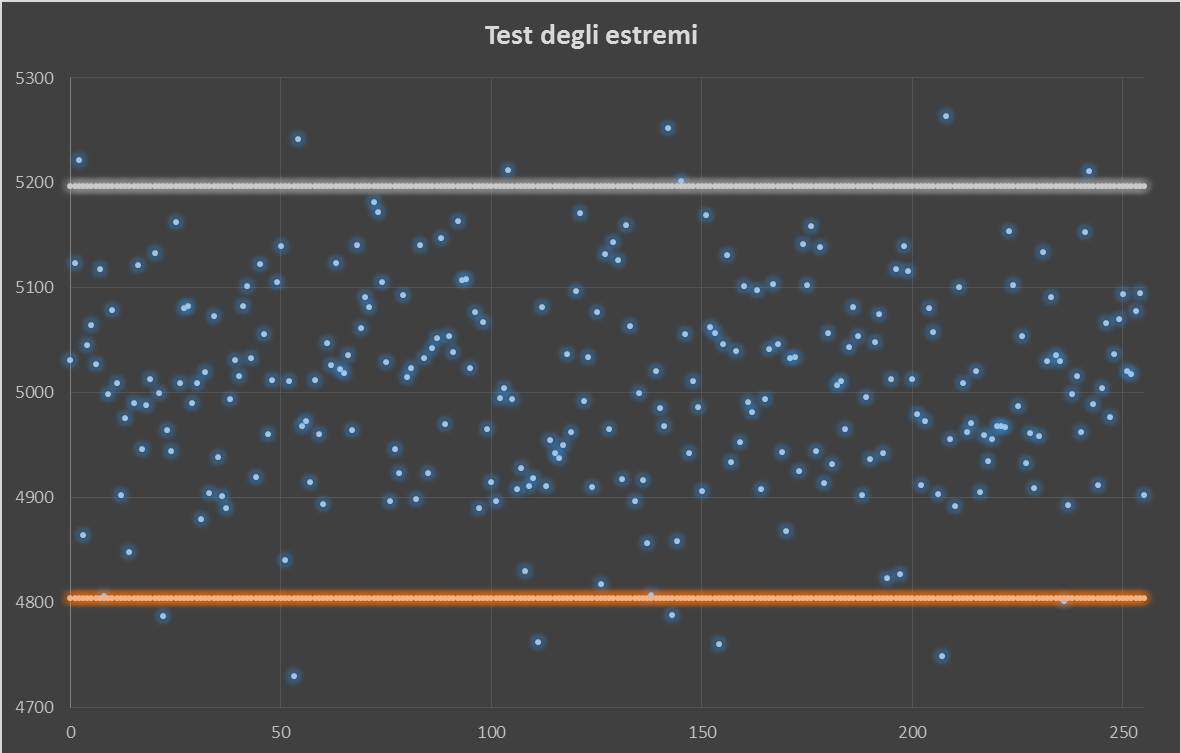
\includegraphics[scale=0.45]{img/test.png}
  \caption[Test degli estremi]{Test degli estremi}
  \end{center}
\end{figure}

\vspace{0.5cm}
I valori critici sono visualizzati come linee orizzontali: quella inferiore rappresenta
$v_1^{*}$ = 4804.92 mentre quella superiore è $v_2^{*}$ = 5196.86

Dalla simulazione effettuata si \'e notato che il numero di test statistici $v > v_2^{*}$ sono stati esattamente 7, come il numero di test $v < v_1^{*}$. Di seguito \'e riportato l'output del programma:

\begin{figure}[H]
  \begin{center}
  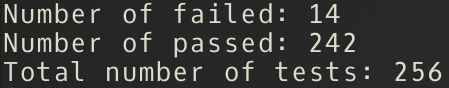
\includegraphics[scale=0.7]{img/test_estremi.png}
  \caption[Risultati]{Risultati}
  \end{center}
\end{figure}


Considerando il numero totale di test falliti (\textit{upper} e \textit{lower bound}) pari a 14, si nota che non
ci si discosta molto rispetto al valore atteso approssimato; infatti in 256 test con un livello di
confidenza del 95\% il valore aspettato è circa 256 * 0.05 = 13 fallimenti. Questo valore pu\`o 
essere una indicazione della bont\`a del generatore di Lehmer implementato.
   	 % 1. Obiettivi
 	\chapter{Obiettivi}
 	\label{cap:obiettivi}
 L'obiettivo del progetto è quello di modellare, pianificare e sviluppare un simulatore di traffico web che rispetti le specifiche di consegna.
 
\vspace{0.5 cm} \noindent Il sistema reale presenta le seguenti caratteristiche:
 \begin{itemize}
 \item un flusso di utenti che si connettono al sistema sotto forma di sessioni;
 \item un numero di richieste di cui si compone ogni sessione;
 \item un front-end server;
 \item un back-end server con un database.
 \end{itemize}

 Il simulatore verr\'a utilizzato per analizzare il comportamento stazionario relativo ad alcuni indici prestazionali quali il tempo di risposta del sistema, il throughput e la percentuale di sessioni abortite e rifiutate.
 Il sistema dispone infatti anche di un meccanismo di \emph{gestione del sovraccarico} basato sul monitoraggio in tempo reale dell'utilizzazione del front-end.\\

% Le specifiche fornite dalla traccia sono le seguenti:
 %\begin{itemize}
 %	\item $\lambda_{sessioni} = 35 \frac{richieste}{s}$ (distribuito esponenzialmente)
 %	\item $Dimensione_{sessioni} \sim Equilikely(5, 35)$
 %	\item $E[Z] = 7 s$ (distribuito esponenzialmente)
 %	\item $E[D]_{front-end} = 0.00456 s$ (distribuito esponenzialmente)
 %	\item $E[D]_{back-end} = 0.00117 s$ (distribuito esponenzialmente)
 %\end{itemize} 
  	 % 2. Modello Concettuale
 	
\chapter{Modello Concettuale}
 	\label{cap:modello concettuale}

Il modello sviluppato è composto da un ramo principale (comprensivo di Front Server, Back-End Server e relative code) e da una componente di retroazione che si compone di un centro di Client, all'interno del quale gli utenti passano un certo tempo a pensare prima di effettuare la richiesta
successiva.

Al sopraggiungere di una nuova sessione, questa verr\'a processata immediatamente dal Front Server, nel caso in cui la sua coda sia vuota, altrimenti verr\'a posta in attesa del proprio turno con un conseguente ritardo. Una volta che il Front Server ha elaborato tale sessione, quest'ultima verr\'a processata all'interno di un Back-End Server, se la coda di quest'ultimo \'e vuota, altrimenti potrebbe subire un certo ritardo dovuto dall'attesa del proprio turno. Al termine di tale servizio la sessione uscir\'a dal sistema, nel caso in cui abbia completato tutte le richieste che la componevano, altrimenti verr\'a reindirizzata nuovamente all'ingresso del sistema attraverso una ramo di feedback.
%All'arrivo di una nuova sessione, questa verr\'a processata dal Front Server, dopo un'eventuale attesa nella sua coda, e successivamente entrerà nel Back-End Server, nuovamente dopo un possibile ritardo di coda. Al termine del servizio la sessione esce dal sistema nel caso in cui abbia completato tutte le richieste che la componevano, oppure rientra nel sistema attraverso un ramo di feedback.%

In tale ramo la sessione permane in un centro di Client in cui l'utente pu\'o spendere del tempo per pensare alla sua richiesta successiva. Dopo tale attesa la sessione tenta di rientrare nel sistema per ricevere un ulteriore servizio, andandosi a posizionare alla fine della coda FIFO del Front Server, inoltre tale servizio \'e senza prelazione ed \'e conservativo.

Il sistema verr\'a regolamentato attraverso un meccanismo di \textit{overload management} che permetter\'a di limitare i tempi di esecuzione della simulazione, nel caso della distribuzione peggiore. Questo consiste nel monitorare l'utilizzazione del sistema implementato, ovvero una volta che abbia raggiunto l' 85\%, il sistema rigetter\'a tutte le richieste (in arrivo e attive), fino a che l'utilizzazione non raggiunga una soglia inferiore al 75\%. Tale tipologia di simulazione garantisce una notevole semplicit\'a di gestione dell'intero sistema attraverso la facilit\'a di avanzamento del tempo ed il controllo delle diverse tipologie di eventi che occorrono durante le varie esecuzioni.

\section{Variabili di Stato}
Il sistema è descritto completamente dalle seguenti variabili di stato:
\begin{itemize}
\item $busy_{fs}^{}$= stato di occupazione del Front Server
\item $queue\_length_{fs}^{}$= numero di richieste nella coda del Front Server
\item $busy\_{bes}^{}$= stato di occupazione nella coda del Back-End Server
\item $queue\_length_{bes}^{}$= numero di richieste nella coda del Back-End Server
\item $client\_counter$= numero di client attivi in un dato istante di tempo

\end{itemize}
Al fine di calcolare medie, varianze, intervalli di confidenza e per visualizzare l'avanzare della simulazione sono state utilizzate anche altre variabili (per lo più booleane o di tipo contatore): \textit{arrivals\, sessions\, requests\, dropped\, aborted\,} $…$ .

\section{Modello delle specifiche}
Nello sviluppo del modello delle specifiche, l'attenzione è stata rivolta alla definizione dei modelli di input da utilizzare nel modello di simulazione. Tali modelli sono stati definiti in base alle specifiche fornite nel seguente modo:

 \begin{itemize}
	\item $\lambda_{sessioni} = 35 \frac{richieste}{s}$ (distribuito esponenzialmente)
 	\item $Dimensione_{sessioni} \sim Equilikely(5, 35)$
 	\item $E[Z] = 7 s$ (distribuito esponenzialmente)
 	\item $E[D]_{front-end} = 0.00456 s$ (distribuito esponenzialmente)
 	\item $E[D]_{back-end} = 0.00117 s$ (distribuito esponenzialmente)
 \end{itemize} 

\section{Eventi}
Dopo aver prodotto un modello delle specifiche sono stati identificati gli eventi generati dal sistema, durante la simulazione:
%Gli eventi che occorrono durante un run del simulatore sono di vario tipo:
\begin{itemize}
\item NewSession: una nuova sessione entra nel sistema. Ovvero verr\'a inserita nel Front Server o nella sua coda qualora quest'ultimo fosse gi\'a occupato;
\item FS\_Completion: il Front Server evade una richiesta e la invia al Back-End Server;
\item BES\_Completion: il Back-End Server evade una richiesta. La sessione corrispondente pu\'o dunque essere completata del tutto e quindi uscire dal sistema oppure migrare verso il centro Client nel caso in cui il suo numero di richieste sia non nullo.
\item Client\_Completion: dopo aver passato un certo tempo in fase di “\textit{Thinking}”, una sessione lascia il centro Client e rientra nel sistema attraverso il ramo di retroazione, quindi \'e direttamente inserita nella coda del Front Server.
\end{itemize}
	 % 3. Generazione numeri random
	\chapter{Modello Progettuale}
	\label{cap:modelloprogettuale}

\section{Architettura}
La struttura associata all'Architettura da implementare pu\'o essere rappresentata semplicemente come in figura \ref{fig:architettura}
\begin{figure}[H]
	\centering
	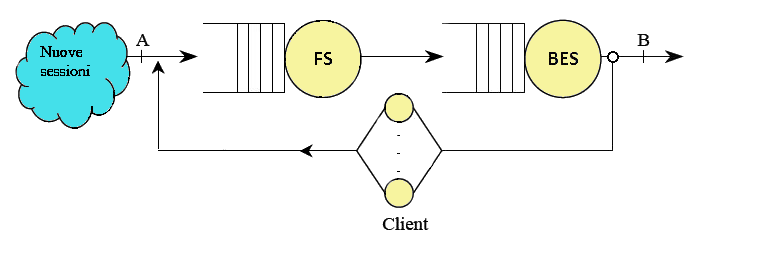
\includegraphics[scale=0.7]{img/architettura.png}
	\caption[Architettura del sistema]{Rappresentazione grafica dell'architettura del sistema.}
	\label{fig:architettura}
	\end{figure}
All'inizio della simulazione il primo evento che si verifica \'e sempre l'arrivo di una nuova sessione (evento NewSession).

\vspace{0.5cm}I client del centro delle sessioni attive, all'interno del ramo di retroazione sono paralleli ed infiniti, definendo un infinity server.

\vspace{0.5cm}Ovviamente i nuovi eventi in arrivo verso il sistema verranno posti in coda al FrontServer, nel caso in cui non possano essere serviti. Come \'e possibile notare nella figura precedente, la sessione una volta servita dal Front Server verr\'a posta in coda verso il Back-End Server finch\'e non verr\'a servita da quest'ultimo. Infine le sessioni saranno completate oppure poste nella zona di "\textit{Thinking}" finch\'e non verranno reinserite nella coda del Front-End in attesa di essere serviti, passando attraverso un ramo di feedback.
 
\section{Clock di simulazione e schedulazione di  Eventi}
Nella fase implementativa si tiene conto dell'avanzamento del tempo per mezzo della variabile \textit{current\_time}. Il meccanismo di avanzamento del tempo scelto \'e il \textit{Next-Event Time Advance}. Questa scelta garantisce che gli eventi occorrano nella sequenza corretta,ovvero vengono processati in ordine crescente rispetto al tempo di schedulazione. Si utilizza, inoltre, il flag di \textit{arrivals} per regolare l'accettazione delle nuove sessioni: se impostata a zero vengono inibiti i nuovi arrivi\footnote{Ovvero viene eseguito il drop della sessione in entrata o l'abort se la sessione \'e gi\'a nel sistema}, altrimenti si procede normalmente con la simulazione.

\section{Event List}
Per la gestione degli eventi si utilizza una lista collegata di strutture \textit{Event}, come quella mostrata in figura, salvate in ordine crescente rispetto al tempo. Ogni nodo contiene il tempo di occorrenza e la sua tipologia. Un gestore di eventi \'e utilizzato per il demultiplexing di tale lista facendo uso di una funzione pop() per ottenere il \textit{Next-Event} da processare.
\begin{figure}[H]
  \centering
  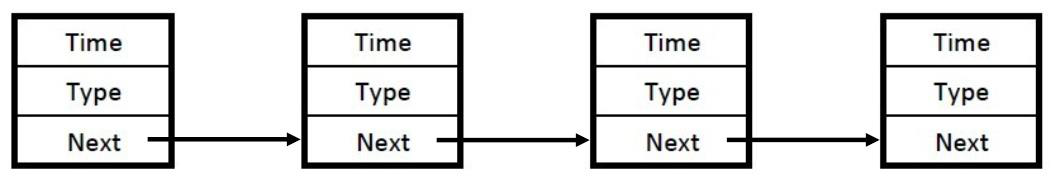
\includegraphics[scale=0.5]{img/EventList.png}
  \caption[EventList]{Struttura lista eventi}
  \label{fig:eventList}
\end{figure}

\section{Arrival Queue}
Al fine di ottenere informazioni riguardo i tempi di attesa che le sessioni sperimentano durante la loro permanenza nel sistema, si utilizzano delle strutture dati atte a registrare tali informazioni ed utilizzate negli algoritmi del calcolo delle medie. Tali strutture, denominate \textit{ArrivalQueue}, immagazzinano i tempi di arrivo delle sessioni nelle sottosezioni del sistema (ovvero quando una sessione entra nel \textit{Front Server} o nella sua coda, quando entra nel \textit{Back-End Server}, e cos\'i via). Ad ogni completamento sperimentato da una sessione viene utilizzata la coda relativa e si calcola, per differenza, il tempo effettivo che la sessione ha passato in quella parte di sistema. Tutto ciò \'e possibile grazie all'ipotesi che l'ordine di arrivo, all'interno delle code del sistema, \'e sempre \texttt{preservato}. Infatti la prima sessione ad entrare nella coda del Front Server, ad esempio, sar\'a la prima a lasciarlo.

\section{Request Queue}
Dal momento che \'e impossibile identificare una singola richiesta utilizzando la Next-Event Simulation, il problema di preservare l'informazione riguardante il numero di richieste attive di cui si compone una sessione viene risolto con la struttura dati \textit{Request Queue}. 

Ad ogni richiesta completata si decrementa il contatore delle richieste relative a quella sessione in modo da propagare tale informazione a tutte le richieste future. Quando il contatore arriva a zero la sessione viene completata del tutto e di conseguenza abbandona il sistema.

\section{Client Order List}
Per preservare una Next-Event Simulation priva di contaminazioni derivanti da una possibile aggiunta di dati identificati delle sessione o delle richieste all'interno degli eventi di base, la Client Order List permette di conservare le informazioni relative all'ordine di arrivo e di uscita  degli utenti all'interno del centro Client. Attraverso questa informazione \'e possibile gestire il corretto ordine degli elementi della Request Queue nonostante siano condizionati da una mancanza di determinismo circa l'ordine di completamento degli utenti durante il loro periodo di Think Time.


\section{Personalizzazione del modello}
In base alle scelte effettuate dall'utente nella fase di \textit{setup} è possibile decidere di avviare la simulazione:
\begin{itemize}
\item senza \textbf{Overload Management}
\item con \textbf{Overload Management}
\end{itemize}
 
\noindent È possibile scegliere quale distribuzione utilizzare tra:
\begin{itemize}
\item \textit{Esponenziale}
\item \textit{10-Erlang}
\item \textit{Iperesponenziale}
\end{itemize}

\noindent \'E poi possibile impostare i parametri riguardanti lo \textit{STOP iniziale, STOP finale e Numero di Run}. Questi parametri sono utilizzati al fine di calcolare il passo\footnote{Per ``\textit{passo}'' si intende l'incremento unitario dell'istante conclusivo di simulazione durante un insieme di run, nel calcolo del comportamento \textit{steady-state}} di ogni esecuzione mediante la seguente formula:

\begin{center}
 $Step = \frac{Stop Iniziale - Stop Finale}{Numero di Run}$
\end{center}

Giunta una nuova sessione, le richieste vengono accodate nel \textit{Front Server} in attesa di essere processate; effettuato il servizio, ovvero verificatosi un evento \textit{FS\_COMPLETION}, tale richiesta passa successivamente al servizio del \textit{Back-End Server}, al termine del quale si verifica un'occorrenza del tipo \textit{BES\_COMPLETION}. 

A questo punto il simulatore valuta per la suddetta sessione il numero di richieste rimanenti ed effettua una scelta: se il numero di richieste per quella sessione \'e zero allora l'utente esce dal sistema; se, al contrario, cos\'i non fosse quest'ultimo attraverser\'a il ramo di feedback per esaurire le proprie richieste rimanenti.

%%Diagrammi per spiegazioni

\section{Avvio e fine simulazione}
Come unico vincolo per il termine della simulazione sono utilizzate due variabili, \textit{START} e \textit{STOP}, che regolano gli orari di apertura e chiusura del sistema.

\noindent Quest'ultimo inizia a schedulare eventi di tipo \textit{NewSession} solo dopo il tempo di \textsc{START} e inibisce tali eventi all'occorrenza del tempo di \textsc{STOP finale}.
\section{Algoritmi di Gestioni eventi}
\subsection{NewSession}
\begin{figure}[H]
  \centering
  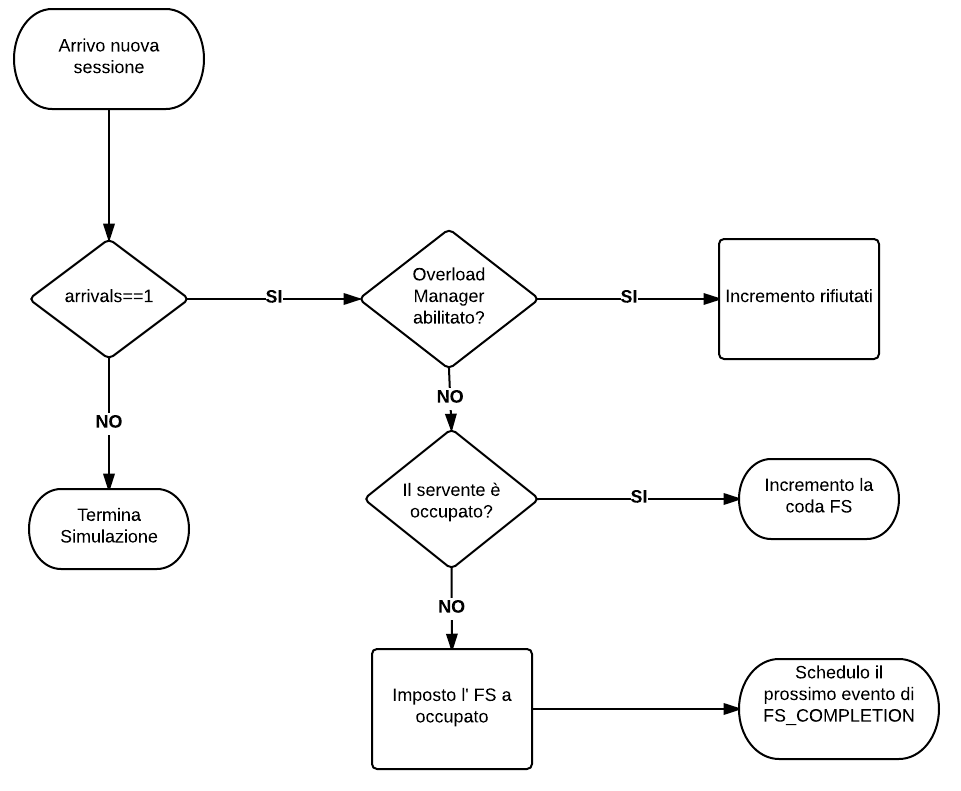
\includegraphics[scale=0.35]{img/NewSession.png}
  %\caption[NewSession]{Struttura lista eventi}
  \label{fig:NewSession}
\end{figure}
\subsection{FS Completion}
\begin{figure}[H]
  \centering
  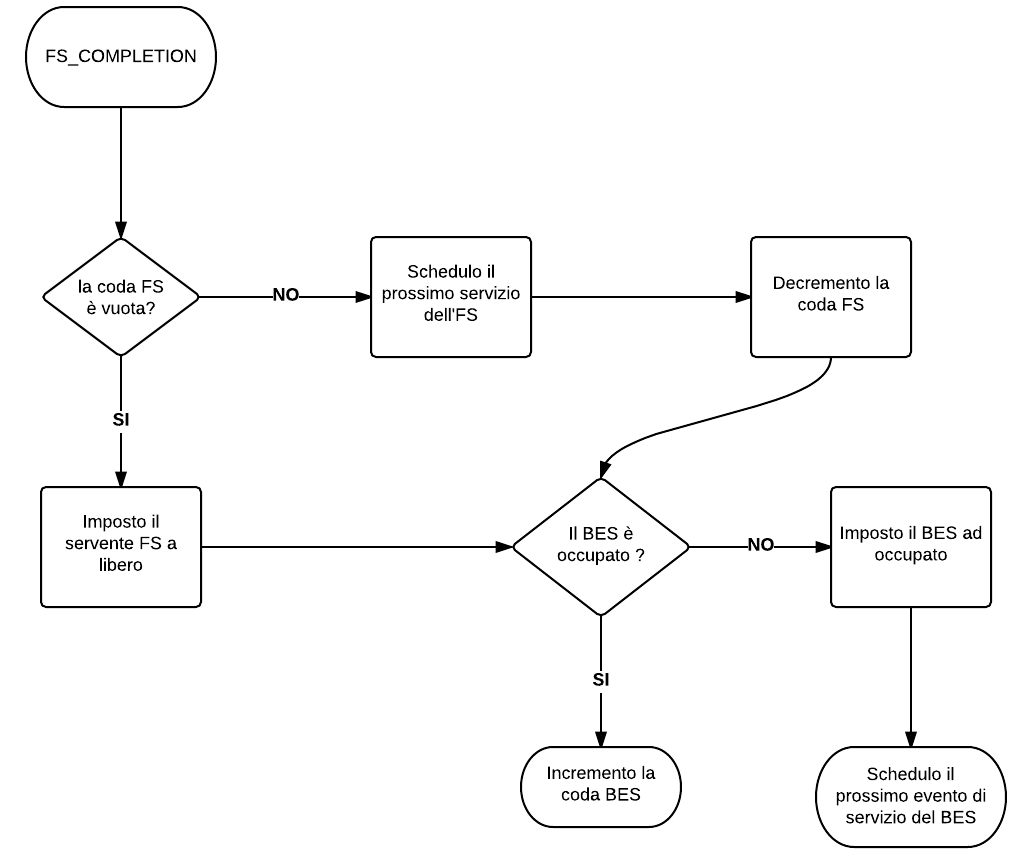
\includegraphics[scale=0.35]{img/FS_Completion.png}
  %\caption[NewSession]{Struttura lista eventi}
  \label{fig:FS_Completion}
\end{figure}

\subsection{BES Completion}
\begin{figure}[H]
  \centering
  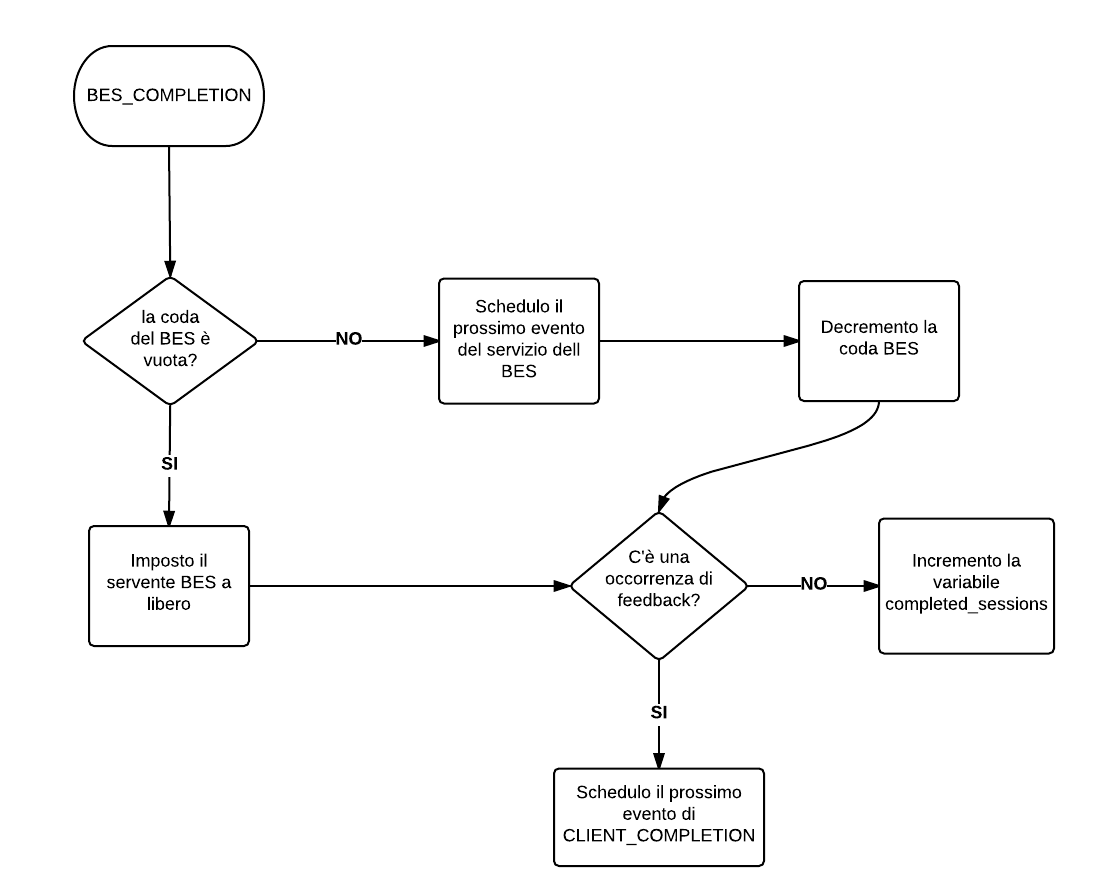
\includegraphics[scale=0.40]{img/BES_Completion.png}
  %\caption[NewSession]{Struttura lista eventi}
  \label{fig:FS_Completion}
\end{figure}

\subsection{Client Completion}
\begin{figure}[H]
  \centering
  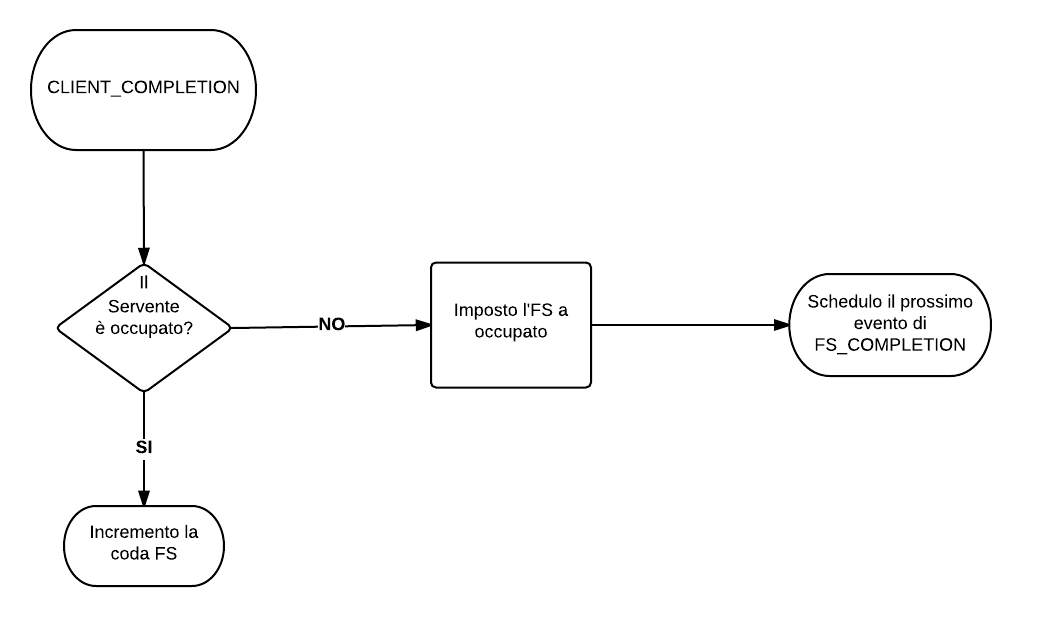
\includegraphics[scale=0.45]{img/CLIENT_Completion.png}
  %\caption[NewSession]{Struttura lista eventi}
  \label{fig:FS_Completion}
\end{figure}
\section{Dati esaminati}
Le richieste progettuali hanno sancito la raccolta di alcuni dati definite da alcune \textit{metriche} quali:
\begin{itemize}
\item \textbf{Troughput}:
\'e l'indice  che misura il totale di sessioni completate nell'unit\'a di tempo. Tale indice viene calcolato attraverso il rapporto tra le sessioni totali processate dal sistema e l'intervallo di tempo necessario per ultimare questo compito.  Il troughput basato sulle sessioni \'e un ottimo indice per valutare il numero di utenti serviti dal sistema in un intervallo dato, risultando una misura sensibile per l'utente finale. Per tener conto della capacit\'a computazionale del sistema data dal numero di singole richieste completate, si \'e deciso di calcolare anche il troughput basato sulle richieste  attraverso un semplice rapporto tra il totale delle richieste processate dal sistema e l'intervallo di tempo utilizzato nell'eseguirle.

\item \textbf{Drop Ratio}:
misura il rapporto tra il totale delle sessioni rifiutate dal sistema ed il numero di sessioni totali che tentano di entrare nel sistema (accettate + rifiutate).

\item \textbf{Abort Ratio}:
\'e il rapporto tra le richieste abortite ed il totale di richieste processate dal sistema.
Questo \'e dovuto dal fatto che una richiesta pu\'o rientrare nel sistema, tuttavia in condizioni di saturazione, tale richiesta non \'e in grado di poter rientrare all'interno del Front Server, quindi viene appunto abortita.

\item \textbf{Tempo di Risposta del Sistema}:
viene inteso come la somma del tempo di risposta (Tempo in coda + Tempo di Servizio) del front-end e del back-end.
In pratica il tempo di risposta \'e inteso come il tempo che intercorre tra l'uscita di una richiesta dal centro di Client, ovvero la fine del periodo di "\textit{Thinking}" di un dato utente, ed il ritorno di tale richiesta al centro.



\end{itemize}
\begin{comment}
\section{Gestione degli eventi}
Vengono riportati nelle figure~\ref{fig:nuovasessione}~\ref{fig:completamentoFE}~\ref{fig:completamentoBE}~\ref{fig:completamentoT} i flussi di esecuzione di ogni evento:
\begin{center}	
	\begin{figure}[H]
	\centering
%	\includegraphics[scale=0.7]{Immagini/arrivo.png}
	\caption[Nuova Sessione]{Nuova Sessione}
	\label{fig:nuovasessione}
	\end{figure}
\end{center}

\begin{center}	
	\begin{figure}[H]
	\centering
%	\includegraphics[scale=0.7]{Immagini/compl_front-end.png}
	\caption[Completamento Front-End]{Completamento Front-End}
	\label{fig:completamentoFE}
	\end{figure}
\end{center}

\begin{center}	
	\begin{figure}[H]
	\centering
%	\includegraphics[scale=0.7]{Immagini/compl_back-end.png}
	\caption[Completamento Back-End]{Completamento Back-End}
	\label{fig:completamentoBE}
	\end{figure}
\end{center}

\begin{center}	
	\begin{figure}[H]
	\centering
%	\includegraphics[scale=0.7]{Immagini/compl_think.png}
	\caption[Completamento Think]{Completamento Think}
	\label{fig:completamentoT}
	\end{figure}
\end{center}
\end{comment}
\begin{comment}
\section{Metriche}
Nella traccia viene richiesto di calcolare le seguenti quattro metriche:
\begin{itemize}
\item Il \textbf{Throughput} è l'indice di prestazione che misura il totale di sessioni completate per unità
di tempo. Tale indice viene calcolato attraverso il rapporto tra le sessioni totali e l'intervallo di tempo necessario per il processamento.
\item Il\textbf{Dropped Ratio} misura il rapporto tra il totale delle sessioni rifiutate dal sistema ed il numero di sessioni totali che tentano di entrare nel sistema (accettate + rifiutate).
\item L'\textbf{Aborted Ratio} è il rapporto tra le richieste abortite ed il totale di richieste processate dal sistema
\item Il \textbf{Tempo di Risposta del sistema} inteso come somma del tempo di risposta\footnote{Tempo in coda più tempo di servizio} del front-end e del back-end.
\end{itemize}
\end{comment}

\section{Modello Analitico}
Al fine di prevedere, in linea di massima, i risultati del simulatore, viene elaborato un modello  analitico semplificato per poter studiare il sistema preso in esame.
Il sistema implementato presenta numerosi vincoli ed una complessit\'a insita nelle specifiche, a tal proposito viene proposto un modello volontariamente e lievemente differente dal caso reale, fornendo un limite inferiore delle prestazioni e degli indici misurati.

Il sistema esaminato risulta essere interattivo, in quanto avviene uno scambio di richieste tra Client e Server, con un comportamento a rete aperta ( le nuove sessioni possono entrare nel sistema qualora questo non fosse saturo), a tal proposito si \'e deciso di presentare due modelli differenti tra loro, uno a rete aperta ed uno a rete chiusa. Questi permettono di descrivere in dettaglio la maggior parte degli elementi che costituiscono il sistema stesso.

\section{Modello semplificato a rete aperta}
In questo primo modello si ha una rete aperta di Jackson con un tasso di sessioni in
arrivo pari a $\gamma$ . Si \'e deciso cos\'i, per questioni di semplificazione del modello, di non
inserire, come componenti, la Priority Queue e il centro di Client, in quanto
risultavano di difficile analisi in un modello di rete aperta come quello di Jackson.
\begin{center}	
	\begin{figure}[H]
	\centering
	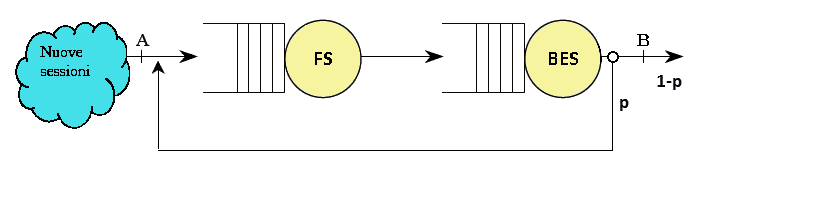
\includegraphics[scale=0.7]{img/reteJackson.png}
	\caption[Modello a rete aperta]{Modello a rete aperta}
	\label{fig:Modello a rete aperta}
	\end{figure}
\end{center}

$\gamma = 35 sessioni/s$

$\vspace{2mm}$

$\begin{cases} 
\lambda_{1} = \gamma + p \lambda_{2} \\ \lambda_{2} = \lambda_{1} \\
\end{cases}$  $\rightarrow$
$\begin{cases} 
\lambda_{1}(1-p) = \gamma \\ \lambda_{2} = \lambda_{1} \\
\end{cases}$ $\rightarrow$
$\begin{cases} 
\lambda_{1} =\frac{ \gamma}{(1- p)} \\ \lambda_{2} =\frac{\lambda_{2}}{(1-p)} \\
\end{cases}$
$\vspace{2mm}$
$\lambda_{1} = \lambda_{2} = \frac{\gamma}{(1-p)} ; p=\frac{19}{20} \rightarrow \lambda_{1} = \lambda_{2} = 35\times20 = 700 richieste/s$
$\vspace{2mm}$

$\lambda_{1}\gg\mu_{FS}; \lambda_{2}=\mu_{FS} poichè \mu_{BES}\gg\lambda_{1}$
$\vspace{2mm}$
 Viene quindi calcolato il throughput, ovvero il numero di sessioni che escono dal sistema al secondo:
$\vspace{2mm}$

$\lambda_{2} =\frac{\lambda_{2}}{(1-p)}=\frac{\mu_{FS}}{20}\approx\frac{219}{20} richieste/s =X_{sessioni}$
$\vspace{2mm}$
$\vspace{2mm}$
$X_{richieste}=X_{sessioni}\times20$
$\vspace{2mm}$
Per quanto concerne l'indice riguardante la percentuale di sessioni rifiutate dal sistema, si trova:
$\vspace{2mm}$

$dropped=\frac{\#sessioni accettate}{\#totale arrivi}$ $\rightarrow$ $\frac{35-X_{sessioni}}{35} = 1-\frac{2}{7}\approx 0.7$ $\rightarrow$ $\%dropped \approx 70\%$

\section{Modello semplificato chiuso}
\begin{center}	
	\begin{figure}[H]
	\centering
	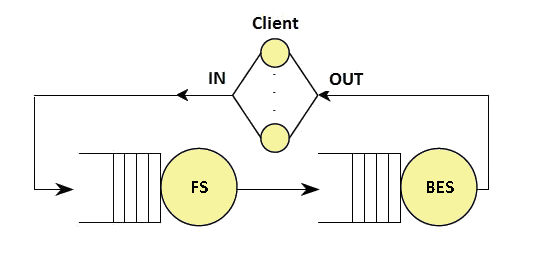
\includegraphics[scale=0.7]{img/retechiusa.png}
	\caption[Modello a rete chiusa]{Modello a rete chiusa}
	\label{fig:Modello a rete aperta}
	\end{figure}
\end{center}

$D_{FS}=0.00456; D_{BES}=0.00117; E[Z]=7s ; N=250$ (in realt\'a il numero aumenta costantemente!).
$\vspace{2cm}\hspace{2mm}$
$\vspace{2mm}\hspace{2mm}$ Anche qui si pu\'o calcolare il throughput del sistema, come:
$\vspace{2mm}$
$X = min\{\frac{1}{D_{max}},\frac{N}{D+Z}\}= min\{\frac{1}{D_{FS}},\frac{250}{D_{FS}+D_{BES}+Z}\}=35.685 richieste/s$.
$\vspace{2mm}$
Da cui si pu\'o ricavare il lower bound per il tempo medio di risposta.
$\vspace{2mm}$
$E[R]\geq max\{D,\frac{N}{X}-E[Z]\}= max \{0.00573,\frac{250}{35}-7\}\approx0.0057447$

	 % 4. Modello delle Specifiche
	\chapter{Modello Computazionale}
Il programma realizzato \'e composto da un file eseguibile (simulatore.c) e di 
alcuni file dove sono contenute funzioni di appoggio. (\textit{event\_list}, 
\textit{arrival\_queue}, \textit{autocorrelation}, \textit{client\_req}, 
\textit{req\_queue}).
Il software sviluppato \'e codificato con il linguaggio \textit{C}.

\section{Simulatore.c}

Questo applicativo \'e il cuore del simulatore implementato. Tale programma 
sfrutta un'interfaccia testuale per interrogare l'utente circa la 
configurazione 
da adottare per la simulazione da eseguire. 
\'E possibile selezionare diverse opzioni:
\begin{itemize}
\item Scegliere la distribuzione da testare;
\item Scegliere se attivare o meno il meccanismo di gestione dell'overload;
\item Scegliere il seed per la generazione di numeri random;
\item Scegliere il tipo di simulazione e i parametri associati;
\item Scegliere se visualizzare lo stato della simulazione live.
\end{itemize}

I risultati prodotti dalla simulazione vengono trascritti su un file di tipo 
"\textit{.csv}"  in modo da dare all'utente una chiara ed equilibrata visione 
dei dati ottenuti.

\section{Event List}
La lista di eventi \'e costituita da strutture di tipo \textit{Event}, formate 
da un campo di tipo \textit{double}, che rappresenta il tempo 
di occorrenza dell'evento, un \textit{\_EVENT\_TYPE} che identifica il tipo di 
evento 
ed un puntatore \textit{next} alla struttura seguente.
Per merito della funzione \textbf{add\_event()} \'e possibile aggiungere eventi 
alla lista. Verranno inseriti seguendo un ordinamento crescente rispetto alla 
variabile time. Durante l'inserimento dei dati viene effettuato un controllo 
sulla consistenza degli stessi, cio\'e si controlla, con una funzione 
\textbf{event\_check()}, che il tempo sia un valore positivo e che il tipo di 
evento appartenga all'insieme degli eventi noti (es: \texttt{nuova sessione}, 
\texttt{fs completition}, ...).     
Gli eventi vengono estratti dalla struttura attraverso la funzione 
\textbf{pop\_event()}, che preleva l'elemento in testa alla lista, 
restituendolo 
alla funzione chiamante.

\section{Arrival Queue}
Definisce una struttura dati, utilizzata per modellare le code sia del Front Server
che del Back-End Server. Ogni coda associata ad un centro si compone di un tempo di arrivo e un puntatore all'elemento successivo. 
Le funzioni messe a disposizione per questa struttura dati sono: 
l'\textbf{arrival\_add()} che aggiunge un nuovo elemento posizionandolo in fondo alla coda, l'\textbf{arrival\_pop()} 
che permette l'estrazione dell'elemento in testa e l'\textbf{arrival\_print()} che stampa lo stato della coda.

\section{Request Queue}
Il sistema all'arrivo di una nuova sessione genera in maniera random,
con distribuzione esponenziale, un numero di richieste comprese tra 5 e 35.
Per evitare di memorizzare tale informazione all'interno della sessione stessa
\'e stata creata, questa struttura dati adibita a raccogliere tali parametri.
Non appena la sessione arriva nel primo centro, ossia il Front Server, il dato 
contenente il numero di richieste associate, viene inserito in questa coda tramite la funzione 
\textbf{enqueue\_req()}. Quando invece la sessione esce dal Back-End Server \'e necessario
l'utilizzo della funzione di \textbf{dequeue\_req()} poich\`e questa informazione non verrà pi\`u
memorizzata in questa lista, ma verr\`a salvata in una diversa struttura, nel caso la sessione non sia completata.
Per verificarne la consistenza \'e stata implementata la funzione \textbf{print\_req()}.

\section{Client request}
Questa struttura dati ci viene in aiuto nel momento in cui la sessione 
esce dal Back-End Server per entrare nel centro di client. In questo caso 
infatti non vengono pi\`u utilizzate le strutture precedentemente descritte,
quali \textit{Request Queue} e \textit{Arrival Queue}, per modellare il comportamento 
del sistema, poich\`e durante la fase di ``thinking'' l'ordine di entrata delle sessioni 
non corrisponde a quello di uscita. Di conseguenza \'è stata creata questa struttura,
che al suo interno contiene sia il tempo di arrivo della sessione nel centro, sia il numero
di richieste rimanenti al suo completamento, per garantire una corretta corrispondenza tra la sessione ed il suo numero di richieste.
Le funzioni di cui dispone questa struttura, sono: 
\textbf{add\_client\_req()}, \textbf{pop\_ClientReq()} e 
\textbf{print\_client\_req()}, esattamente identiche a quelle delle strutture 
precedenti.

\section{File Manager}
La parte relativa al file manager gestisce tutto il flusso di dati da 
trascrivere  su un file di output. Composto da tre funzioni:
\begin{itemize}
\item \textbf{get\_date()}: permette di ottenere l'orario e la data correnti, 
da 
salvare sul file desiderato.
\item \textbf{open\_file()}: utilizzata per la creazione e l'apertura 
del file da salvare. Il nome del file viene creato sfruttando la funzione 
\textbf{get\_date()}. Quindi il file contiene la data corrente della creazione pi\`u il 
tipo di 
distribuzione scelta durante la fase di setting.
\item \textbf{close\_file()}: adottata per chiudere il file una volta 
terminata la scrittura su di esso.
\end{itemize}

\section{Utils}
Il file \textbf{utils.h} contiene delle funzioni utilizzate per la pulizia della 
console 
e alcune funzioni per la manipolazione dei dati ottenuti al termine della 
simulazione.

\begin{comment}
\section{Autocorrelazione}
Al fine di calcolare l'autocorrelazione sui tempi di risposta del sistema con 
\textbf{LAG} pari a 20 \'e stato scritto un programma C che prende in input il 
file generato dal simulatore e restituisce i valori calcolati delle 
autocorrelazioni. Per il calcolo di queste si \'e usata la formula:

\vspace{0.5cm}
\begin{center} $r_{j} = \frac{c_{j}}{c_{0}} con j = 1,2,...20$\end{center}

\section{Intervalli di confidenza}
\'E stato sviluppato un programma scritto in linguaggio \textbf{C} allo scopo 
di 
calcolare gli intervalli di confidenza di livello 1 - \textalpha, dove 
\textalpha è pari al 5\%. Tale programma prende in input un file in cui sono 
scritti tutti i valori su cui si vuole fare il calcolo e computa le seguenti 
statistiche:
\begin{itemize}
 \item Calcolo della media: $\bar{x}_{i} = \frac{1}{i}(x_{i} - \bar{x}_{i-1})$;
 \item Calcolo della varianza: $v_{i} = v_{i-1} + (\frac{i-1}{i}){(x_{i} - 
\bar{x}_{i-1})}^{2}$;
 \item Calcolo del valore critico: $t^{*} = idfStudent(n-1, 
1-\frac{\textalpha}{2})$;
 \item Calcolo degli estremi dell'intervallo: $\bar{x} \pm 
\frac{t^{*}s}{\sqrt{n-1}}$;
\end{itemize}
\end{comment}     % 5. Modello Computazionale
 	\chapter{Verifica}

La fase di verifica \'e molto importante poich\'e consente di dimostrare la 
consistenza del programma creato con il modello delle specifiche.

\vspace{0.3cm}In primis, \'e stata utilizzata una funzione di stampa per 
verificare il corretto flusso delle sessioni all'interno dell'intero sistema. 
Tale funzione, la \texttt{print\_system\_state()}, stampa le statistiche pi\`u 
importanti del sistema in tempo reale su standard output.

\vspace{0.3cm}In secundis, si \'e notato e verificato che le liste contenenti le 
sessioni e le richieste si riempiono e si svuotano in modo corretto. Anche in 
questi casi sono state necessarie funzioni di stampa per verificare che 
l'aggiornamento fosse adeguato.

\vspace{0.3cm}In terzis, i vincoli sullo stato del sistema e sull'entrata in 
azione dell'overload manager, e sul calcolo delle medie sono tutti soddisfatti.

\vspace{0.3cm}Il simulatore parte con il numero di sessioni nullo e tutte le 
variabili di stato e di supporto sono inizializzate opportunamente. Il 
sistema consente di avere una stampa aggiornata di tutti i parametri 
rilevanti, come throughput e tempo medio di risposta.

\vspace{0.3cm}Il numero di sessioni rifiutate e abortite cresce in maniera 
consistente con il meccanismo di controllo delle ammissioni.
\begin{comment}
Nel caso in cui l'utente non utilizzi l'overload management, \'e stato dimostrato che superato il tempo di
STOP finale, chiamato FIN all'interno del codice, nessuna nuova sessione
sarebbe stata accettata dal sistema e, successivamente la simulazione
sarebbe stata interrotta perch\'e la coda tenderebbe a crescere all'infinito.
\end{comment}
\vspace{0.3cm}Infine, come ultima verifica, \'e stato dimostrato che superato il 
numero massimo di sessioni per batch, che l'utente ha inserito manualmente, il sistema passa a simulare il batch
successivo, e una volta raggiunto il numero massimo di batch, impostati sempre dall'utente, il programma termina
correttamente la propria esecuzione.

     % 6. Verifica
 	\chapter{Validazione} 

In questa fase viene testata la corrispondenza del simulatore con il modello reale. Sono stati effettuati i seguenti controlli:

\begin{itemize}
 \item Saturazione del Front Server: ci sono due concause che portano alla saturazione del Front Server, in primo luogo c'\'e una enorme differenza tra il tasso di servizio di quest'ultimo e quello del Back-End Server che \'e circa 3 volte maggiore; inoltre il numero di utenti che stazionano nel centro Client tende a crescere enormemente e tale comportamento influenza l'andamento di richieste in entrata al Front Server che ne determina la congestione.
 
 \item La coda del Back-End Server risulta essere quasi sempre vuota poich\'e \'e il Front Server che elabora in maniera lenta mentre il tasso di servizio in questo caso \'e di oltre 800 richieste / secondo; questo non permette la creazione di coda e di conseguenza l'utilizzazione \'e molto bassa.
 
 \item Il numero di client \'e notevolmente elevato: questo \'e dovuto all'elevato Think Time sperimentato dagli utenti, circa 7 secondi a client. Considerando il throughput del sistema ed i tassi di servizio dei due serventi \'e immediato notare come il numero dei client attivi contemporaneamente tenda a crescere nel tempo. Tale componente è modellato come un Infinite Server.
 
 \item Nel caso di overload management la percentuale delle connessioni rifiutate e abortite \'e molto alta arrivando a toccare anche l'87\% nel secondo caso, mentre nel primo \'e pi\'u contenuta, con un massimo che si attesta circa attorno al 30\% per poi oscillare in quell'intorno. Questo perch\'e il Front Server rappresenta il collo di bottiglia dell'intero sistema.
\end{itemize}     % 7. Validazione
 	\chapter{Progettazione Esperimenti e Simulazioni} 

Tutte le simulazione sono state effettuate su diversi computer, sia Pc desktop 
che notebook, sfruttando la portabilit\`a del software in modo tale da generare 
i dati sia su sistemi operativi \textit{Windows} che \textit{Linux}. La 
simulazione viene testata con parametri inseriti dall'utente manualmente, 
permettendo una facile impostazione del programma.
Sono state sfruttate macchine aventi processori multi-core al fine di eseguire 
pi\`u esecuzioni in parallelo.

\noindent Gli esperimenti eseguiti sono stati i seguenti:

\begin{enumerate}
 \item Simulazione del sistema quando il Front Server ha distribuzione 
esponenziale;
 \item Simulazione del sistema quando il Front Server ha distribuzione 
10-Erlang;
 \item Simulazione del sistema quando il Front Server ha distribuzione 
Iperesponenziale;
 \item Simulazione del sistema nel caso peggiore tra i precedenti con overload management attivo.
\end{enumerate}

\noindent \vspace{0.5cm} Gli esperimenti sono stati basati sui seguenti 
parametri:
\begin{itemize}
 \item \textbf{\textit{Seed}} : indica il seed scelto dall'utente nella fase di setup;
 \item \textbf{\textit{Batch size}} : indica quante sessioni compongono un batch;
 \item \textbf{\textit{Batch number}} : indica quati batch devono essere eseguiti in totale;
 \item \textbf{\textit{Threshold}} : indica se l'overload management \'e attivo.
\end{itemize}

Per ogni simulazione si \'e scelto di impostare la grandezza del \textit{batch} 
ed il suo numero di esecuzioni con lo stesso valore in modo da poter effettuare
un miglior confronto tra i diversi casi. Al termine di ogni \textit{batch} i dati 
ottenuti dalle metriche considerate vengono salvati su un file ``\textit{csv}''.
Al termine di tutti i \textit{bach} vengono computati e salvate su file ulteriori 
informazoni relative all'esecuzione generale, come ad esempio l'autocorrelazione o
gli intervalli di confidenza.     % 8. Progettazione Esperimenti
 	\chapter{Analisi dei Risultati} 

I dati relativi agli indici di prestazione di interesse (tempi di risposta e 
throughput) misurati 
nelle precedenti fasi di test sono stati in seguito aggregati e visualizzati in 
forma di grafici. 
Infatti, in base al tipo di test effettuato, tali grafici si suddividono in due 
categorie: i grafici di 
throughput e tempi di risposta del sistema in stato di instabilit\`a (front 
server sovraccarico) e 
quelli relativi al sistema in condizione di stazionariet\`a (front server non 
sovraccarico), ovvero quelli gestiti
attraverso il meccanismo di overload management.

\section{Sistema senza Overload Management}

\subsection{Response Time}

In questo scenario l'utilizzazione del front-end server \'e praticamente uguale 
a 1, perci\`o 
non riesce a completare tutte le richieste entranti, con la inevitabile 
situazione di veder aumentare indefinitamente la lunghezza della sua coda. Di 
conseguenza il tempo di risposta del sistema tende a divergere all'aumentare del 
tempo di 
simulazione. Il grafico illustrato di seguito mostra tale scenario:

\begin{figure}[H]
 \centering
 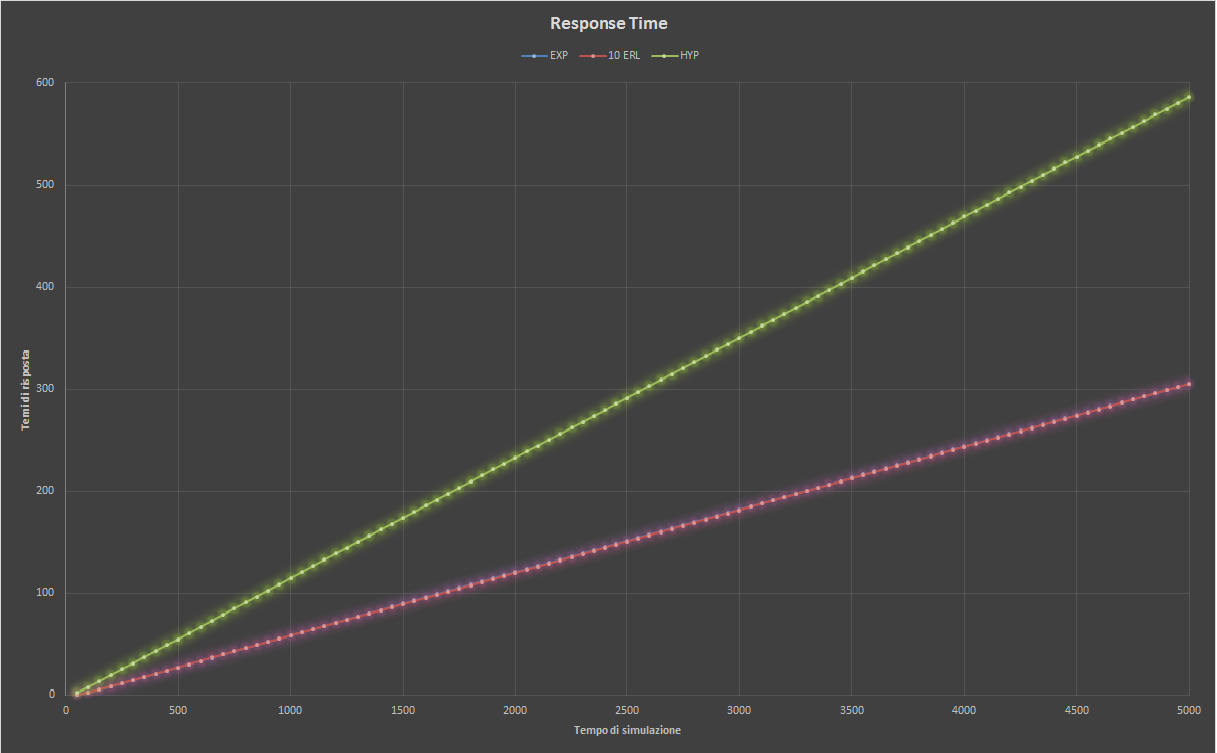
\includegraphics[scale=0.45]{img/responseTime.png}
 \caption[Tempi di risposta del sistema instabile]{Tempi di risposta del sistema 
instabile}
 \label{fig:Tempi di risposta del sistema instabile}
\end{figure}

Come si intuisce dal grafico sopra riportato, i tempi di risposta si 
contraddistinguono in base
al tipo di distribuzione dei tempi di servizio del front-end server 
(iperesponenziale, 10-erlang 
ed esponenziale), e in base all'andamento delle curve dei tempi di risposta, 
risulta evidente 
come la distribuzione iperesponenziale dei tempi di servizio del front-end 
risulta peggiore 
che nel caso esponenziale e 10-erlang, dove i tempi rimangono uguali.

Questa sostanziale differenza \`e dovuta al fatto che, nel caso 
iperesponenziale, avendo 
preimpostato la probabilità \textbf{p=0.1}, la varianza dei tempi di servizio 
delle richieste risulta 
essere molto elevato con la conseguenza di rallentare notevolmente il front-end 
server.
Di conseguenza la curva dei tempi di risposta della iper-esponenziale diverge 
pi\`u 
rapidamente rispetto alle controparti 10-erlang ed esponenziale. Tuttavia il 
grafico mostra 
anche un aspetto insolito: la curva del tempo di risposta della 10-erlang 
coincide 
praticamente con la curva dell'esponenziale anche avendo impostato un parametro 
K=10, 
mentre ci si aspettava, al contrario, un miglioramento dei tempi di risposta 
rispetto alla curva 
della esponenziale. Probabilmente la scelta del parametro K pari a 10 \'e 
insufficiente a 
garantire un miglioramento significativo.

\subsection{Autocorrelazione}

L'evidente divergenza dei tempi di risposta del sistema \'e evidenziata anche 
dalla forte 
correlazione presente dai tempi di risposta delle singole richieste presenti nel 
sistema. Il 
grafico seguente illustra tale correlazione sulle tre distribuzioni:

\begin{figure}[H]
 \centering
 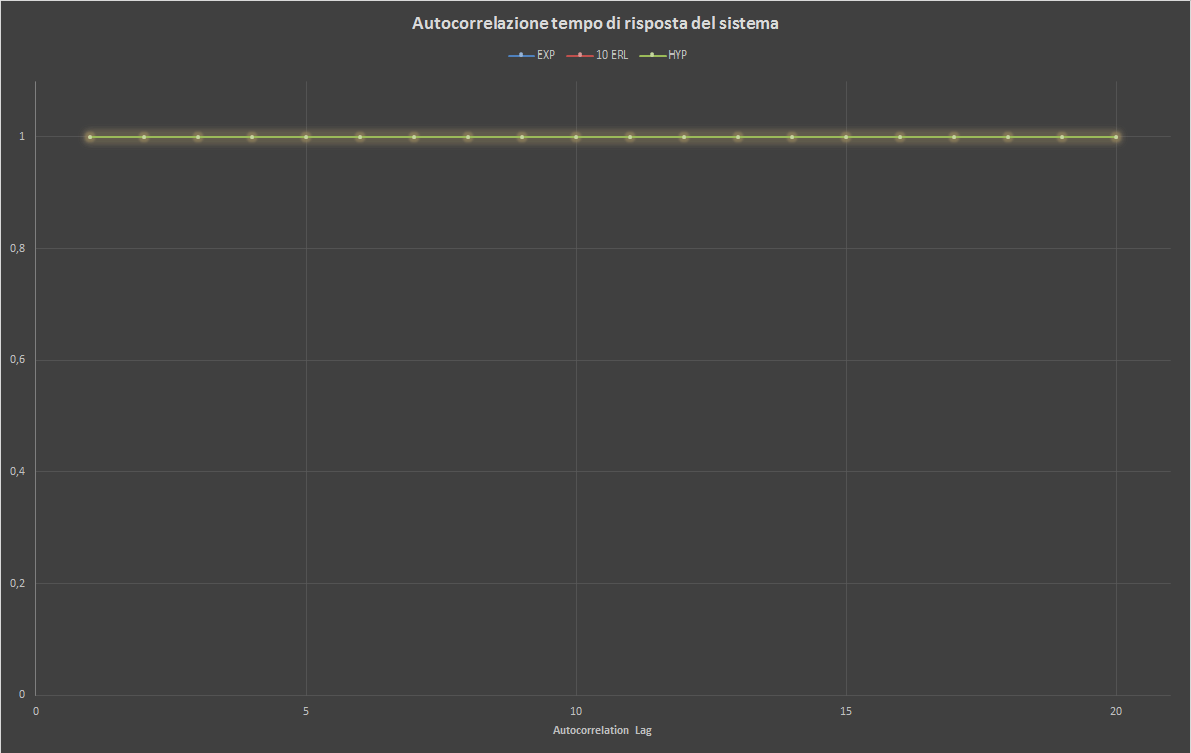
\includegraphics[scale=0.45]{img/autocorrelation.png}
 \caption[Autocorrelazione dei tempi di risposta]{Autocorrelazione dei tempi di 
risposta}
 \label{fig:Autocorrelazione dei tempi di risposta}
\end{figure}

Dal grafico non si evince bene ma i valori dell'autocorrelazione relativi alla 
distribuzione
iperesponenziale sono leggermente inferiori rispetto agli altri due casi 
(nell'ordine di $10^{-2}$)
ma si assestano tutti nell'intorno di 0.9.

\subsection{Useful Throughtput}

Il grafico successivo mostra l'andamento dello useful throughput i cui valori 
sono stati
misurati dagli stessi test usati per il tempo di risposta del sistema. Anche in 
questo caso si 
distinguono le diverse distribuzioni dei tempi di servizio del front-end server:

\begin{figure}[H]
 \centering
 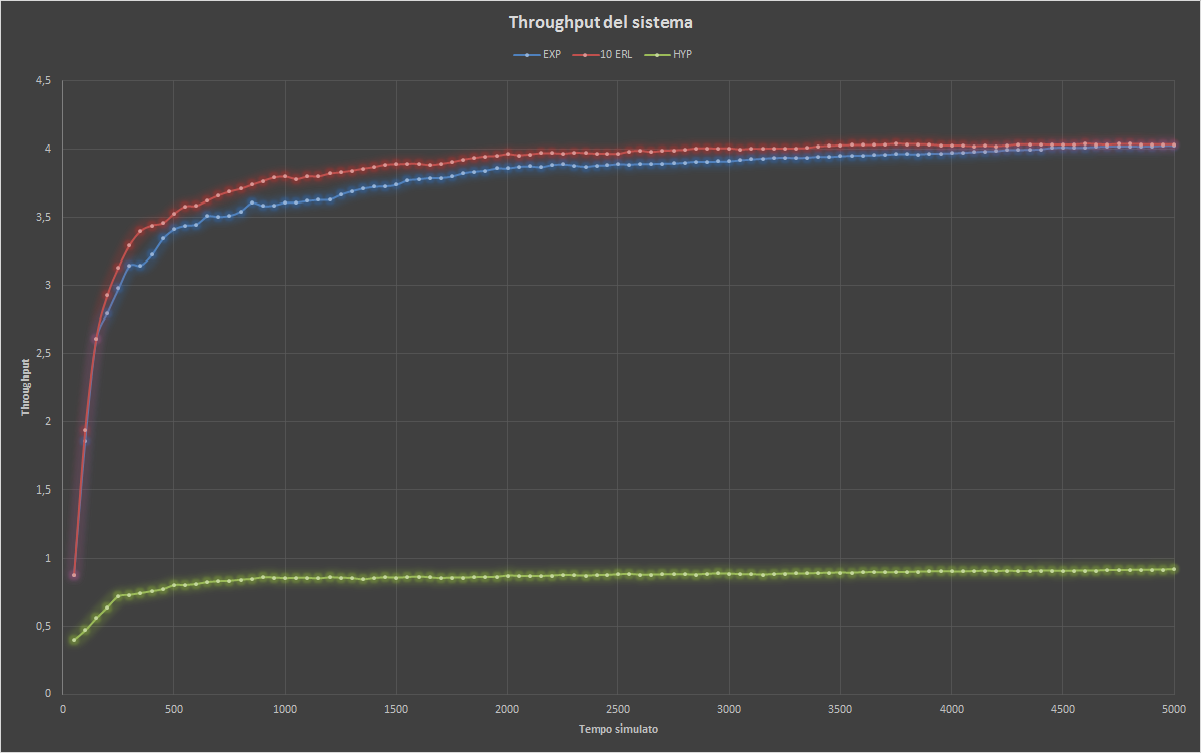
\includegraphics[scale=0.45]{img/throughput.png}
 \caption[Throughput del sistema instabile]{Throughput del sistema instabile}
 \label{fig:Throughput del sistema instabile}
\end{figure}

Anche in questo caso si nota la notevole differenza dello useful throughput  del 
caso 
iperesponenziale da quelli esponenziali e 10-erlang, i quali coincidono per 
valori di run  
simulativi molto alti.
Lo useful throughput \'e l'unico indice di prestazione che presenta un andamento 
stazionario 
all'aumentare del tempo di simulazione. Si pu\`o notare dal grafico, infatti, 
che tale valore di 
stazionariet\`a \'e all'incirca pari a 4 sessioni completate per unit\`a di 
tempo.


Di seguito sono stati riportati gli intervalli di confidenza stimati per ogni 
distribuzione. 
\begin{itemize}
 \item \textit{\textbf{Esponenziale}} : $[ 3,66109876 ; 3,83534225 ]$
 \item \textit{\textbf{10 Erlang}} : $[ 3,75592814 ; 3,92657294 ]$
 \item \textit{\textbf{Iperesponenziale}} : $[ 0,84149673 ; 0,87406350 ]$
\end{itemize}

Infine viene riportato l'istogramma relativo allo useful throughput dato che 
l'unico
indice con comportamento steady-state:

\begin{figure}[H]
 \centering
 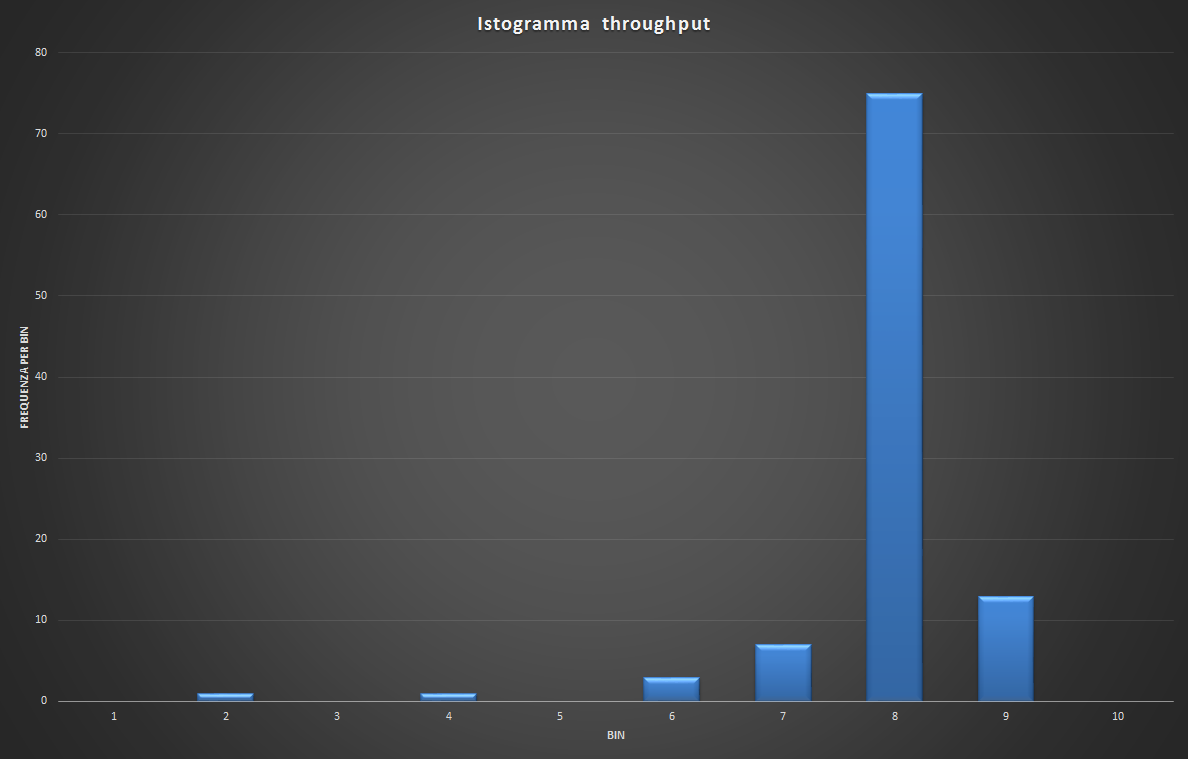
\includegraphics[scale=0.45]{img/istogramma.png}
 \caption[Istogramma del throughtput]{Istogramma del throughtput}
 \label{fig:Istogramma del throughtput}
\end{figure}

\section{Sistema con Overload Management}

Dai risultati illustrati nel caso di sistema senza il meccanismo di 
\textit{overload 
management} la distribuzione con i tempi di servizio ``peggiore'', ossia con i 
tempi
di risposta maggiori, \'e risultata quella iperesponenziale. 
Per questa distribuzione, dunque, sono stati effettuati test con la gestione del 
sovraccarico.
Neanche quando viene applicato l'overload management nel front-end server, gli 
indici di prestazione
di interesse assumono un comportamento stazionario per run simulativi abbastanza 
lunghi.
Ci\`o avviene perch\'e anche se in questa situazione, il front server ha 
un'utilizzazione media pi\`u bassa
di 1, e quindi non arriva mai a saturazione, nel momento in cui supera l' 85\% 
del carico viene impedito l'accesso
a tutte le sessioni, anche quelle gi\`a presenti nel sistema, e di conseguenza 
la sua coda si svuota, ma
nel momento in cui vengono riabilitati gli arrivi la coda si riempie di nuovo, 
con l'effetto che tutte le
metriche analizzate avranno oscillazioni non indifferenti rispetto al tempo.

\subsection{Response Time}

Di seguito viene riportato il grafico sul tempo di risposta del sistema con 
distribuzione dei 
tempi di servizio iperesponenziale del front-end server:

\begin{figure}[H]
 \centering
 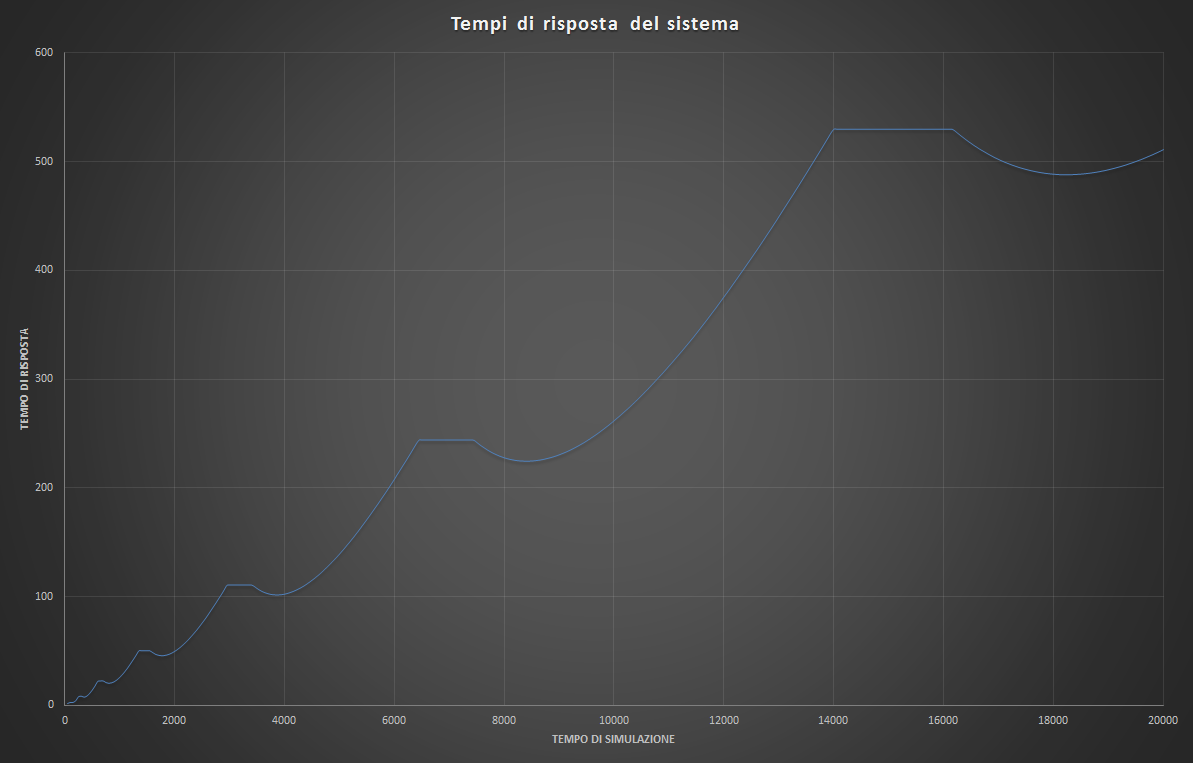
\includegraphics[scale=0.45]{img/responseOM.png}
 \caption[Tempo di risposta del sistema con distribuzione iperesponenziale e 
overload management attivo]{Tempo di risposta del sistema con distribuzione 
iperesponenziale e overload management attivo}
 \label{fig:Tempo di risposta del sistema con distribuzione iperesponenziale e 
overload management attivo}
\end{figure}

Dal grafico riportato sopra, si nota ci\`o che era stato detto in precedenza, 
ovvero il response time
non si stabilizza, ma tende a decrescere nei momenti in cui il sistema blocca 
gli accessi ed a crescere di 
nuovo quando vengono nuovamente abilitati.

\subsection{Useful Throughtput}
Il grafico successivo illustra l'andamento dello useful throughput del sistema 
con i 
parametri sopra citati:
\begin{figure}[H]
 \centering
 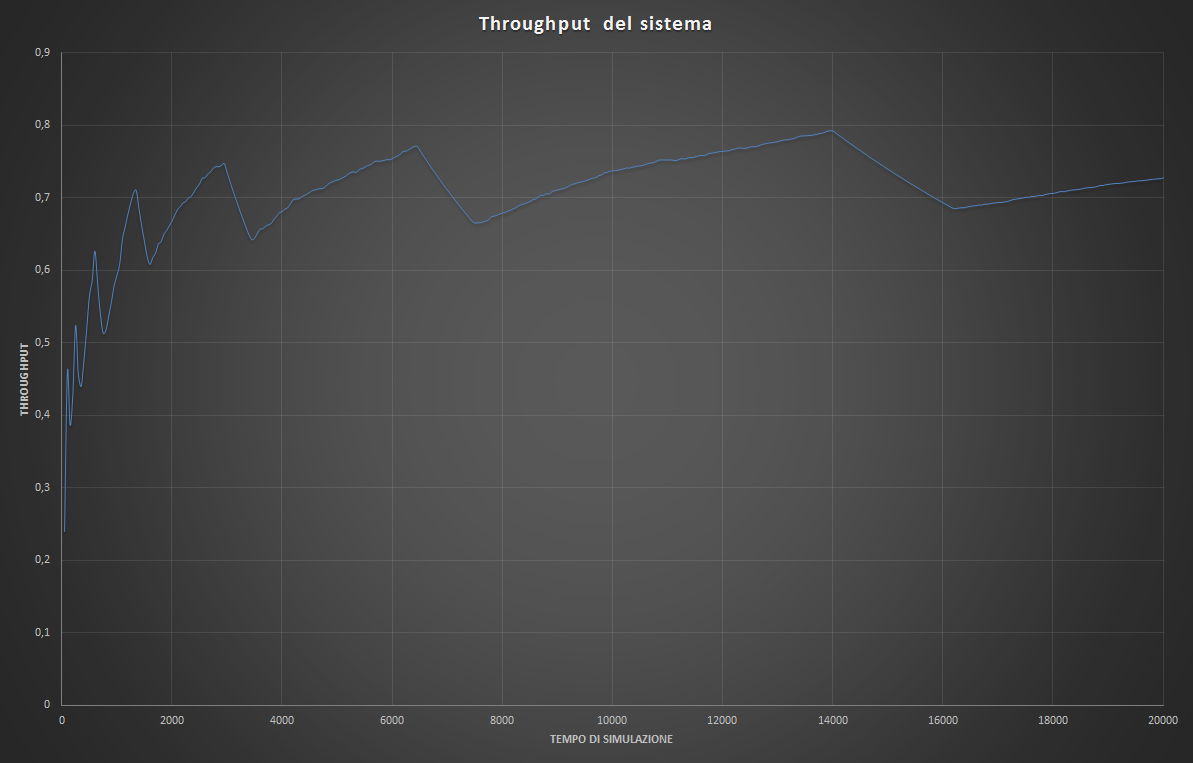
\includegraphics[scale=0.45]{img/throughputOM.png}
 \caption[Throughput del sistema con distribuzione iperesponenziale e overload 
management attivo]{Throughput del sistema con distribuzione iperesponenziale e 
overload management attivo}
 \label{fig:Throughput del sistema con distribuzione iperesponenziale e overload 
management attivo}
\end{figure}
Come \`e possibile notare, nell'analisi del throughput avviene un comportamento 
conforme con quello osservato per i tempi di risposta, anche se in questo caso 
a poco a poco le oscillazioni si vanno ad appiattire.

\subsection{Drop e Aborted Ratio}
Infine vengono riportati gli andamenti degli indici \textit{drop ratio} e 
\textit{aborted ratio}:
\begin{figure}[H]
 \centering
 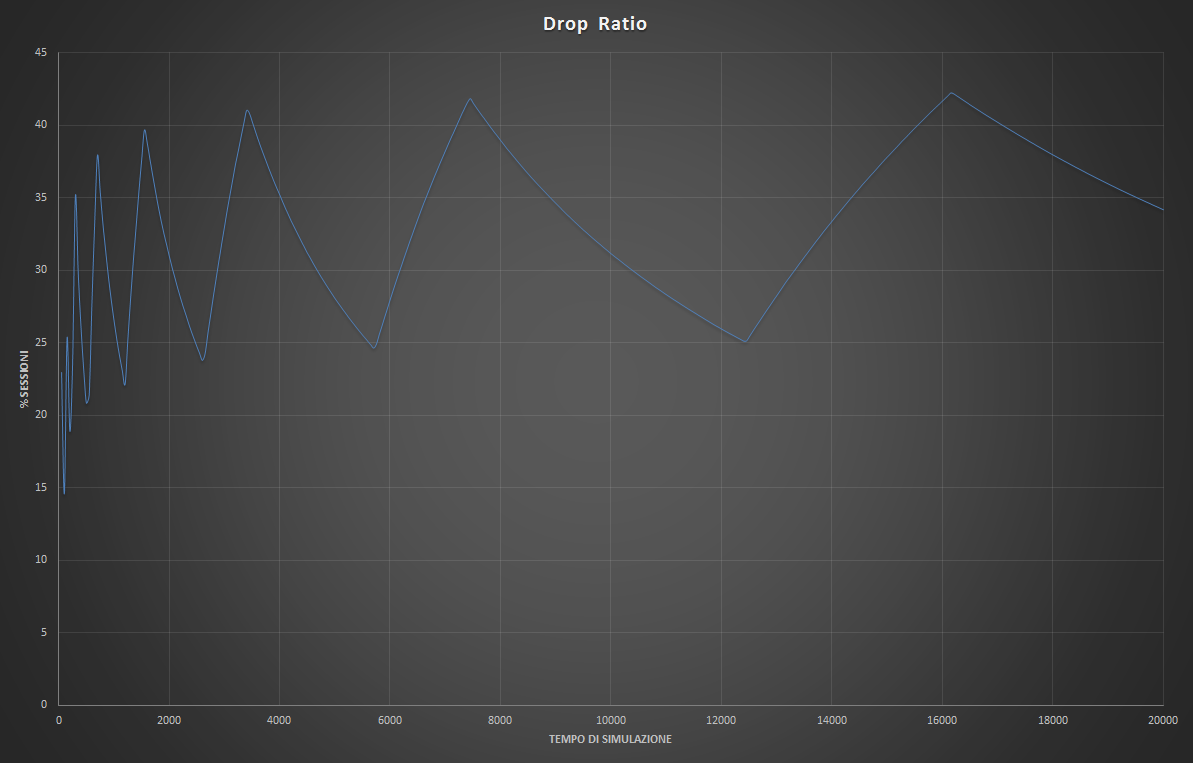
\includegraphics[scale=0.4]{img/dropRatio.png}
 \caption[Drop Ratio]{Drop Ratio}
 \label{fig:Drop Ratio}
\end{figure}
\begin{figure}[H]
 \centering
 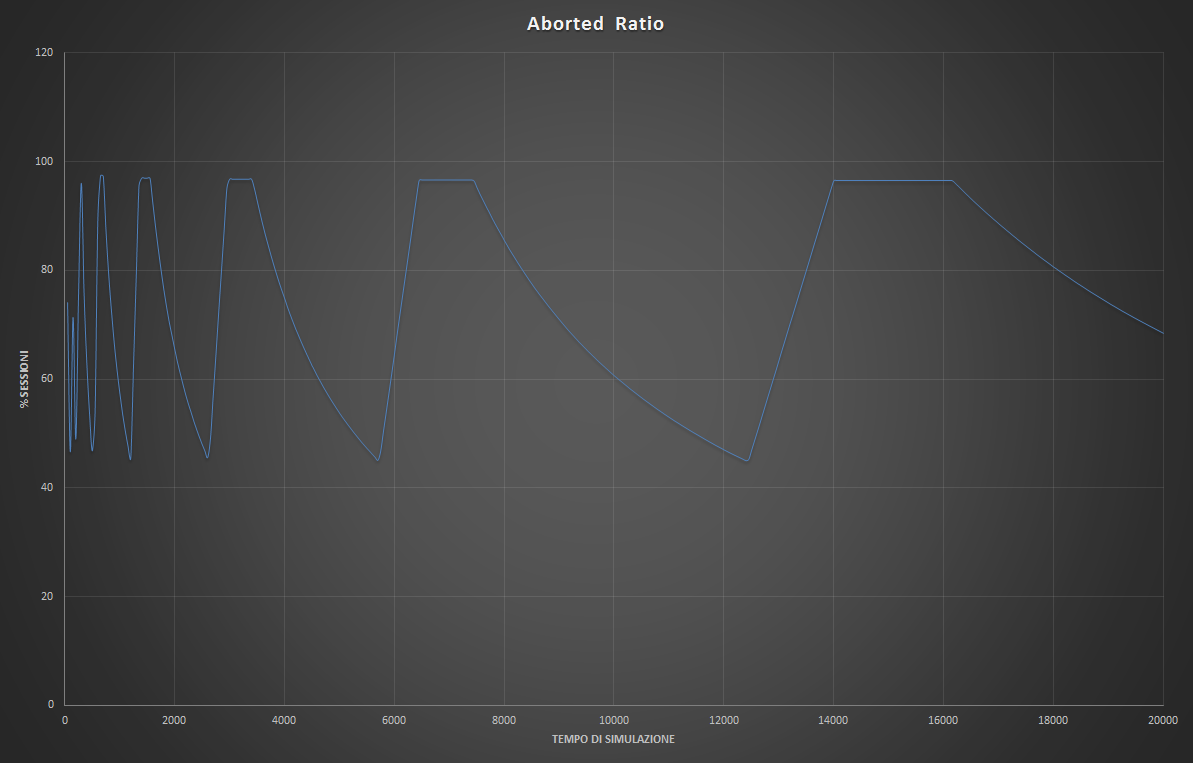
\includegraphics[scale=0.4]{img/abortRatio.png}
 \caption[Aborted Ratio]{Aborted Ratio}
 \label{fig:Aborted Ratio}
\end{figure}
Anche in questi due grafici notiamo come la percentuale di sessioni rifiutate e 
abortite oscilli in maniera molto ampia ed evidente.

\section{Batch means e intervalli di confidenza}

Pur non avendo raggiunto la stazionariet\`a neanche con il meccanismo di overload
management attivo si \'è scelto di eseguire gli stessi test con il metodo dei batch
means. Questo metodo prevede effettuare un unico lungo run e partizionare i dati raccolti relative 
alle statistiche di interesse in partizioni (batch) di uguale lunghezza, calcolare le medie di 
ciascun batch, e successivamente calcolare la media delle medie dei batch, ricavando 
anche la deviazione standard relativa per poter costruire gli intervalli di confidenza per la 
media. Particolare attenzione è stata prestata nella scelta dei parametri (b,k) necessari per 
determinare l’ampiezza e il numero dei batch. Seguendo le linee guida del libro si \'e scelto 
di impostare un k=64 fisso mentre b è stato determinato dal rapporto b=n/k.
Il valore calcolato di b è risultato ottimale anche controllando l’andamento della funzione di 
autocorrelazione (tendente a zero):

\begin{figure}[H]
 \centering
 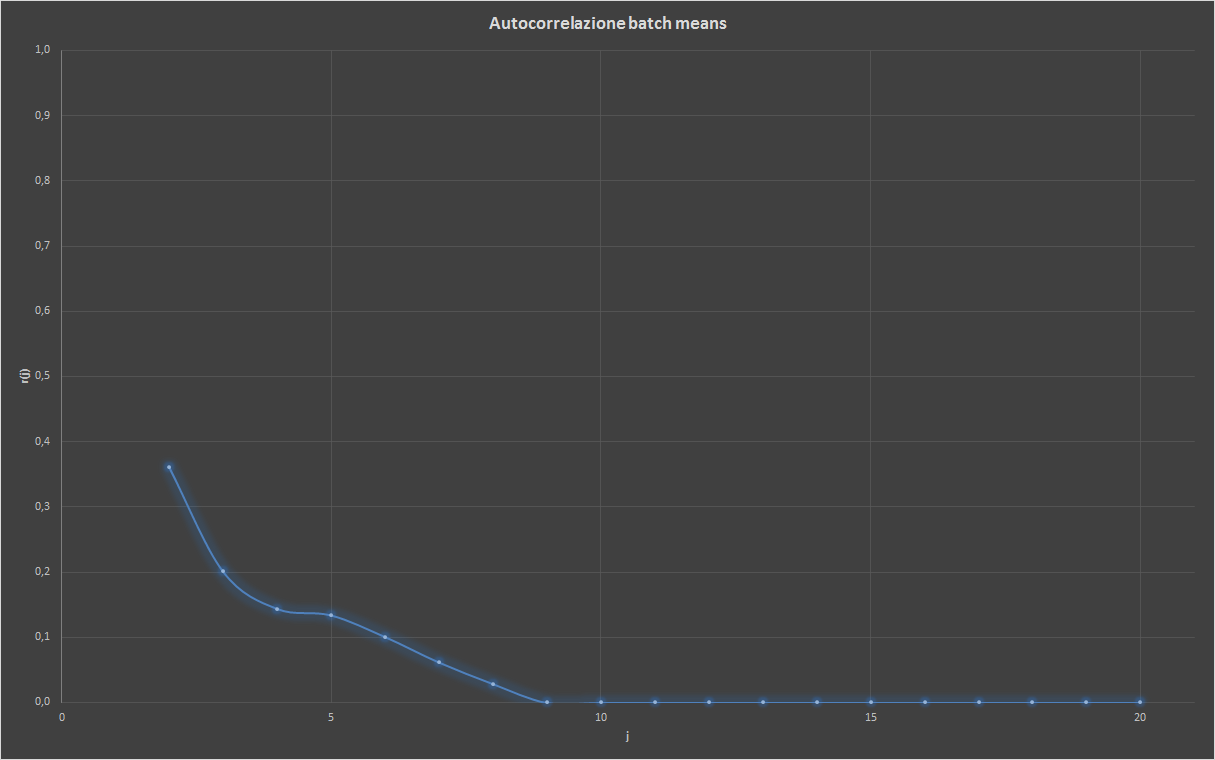
\includegraphics[scale=0.45]{img/autocorrBM.png}
 \caption[Autocorrelazione batch means]{Autocorrelazione batch means}
 \label{fig:Autocorrelazione batch means}
\end{figure}

Nell'analisi effettuata in questo caso si può osservare, dal grafico successivo, come il tempo
di risposta del sistema si stabilizzi e di conseguenza \'e risultato possibile calcolare un intervallo
di confidenza al 95\%. 

\begin{figure}[H]
 \centering
 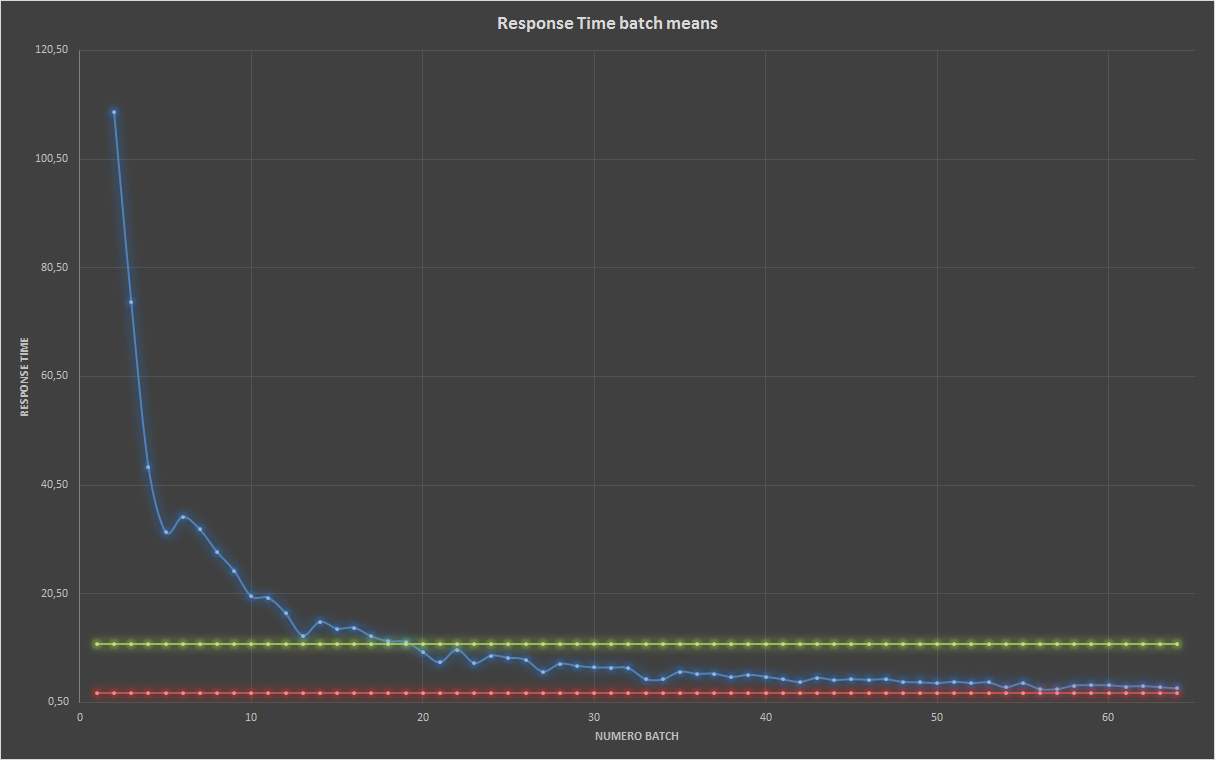
\includegraphics[scale=0.4]{img/resTimeBM.png}
 \caption[Response time nel caso dei batch means]{Response time nel caso dei batch means}
 \label{fig:Response time nel caso dei batch means}
\end{figure}

\begin{figure}[H]
 \centering
 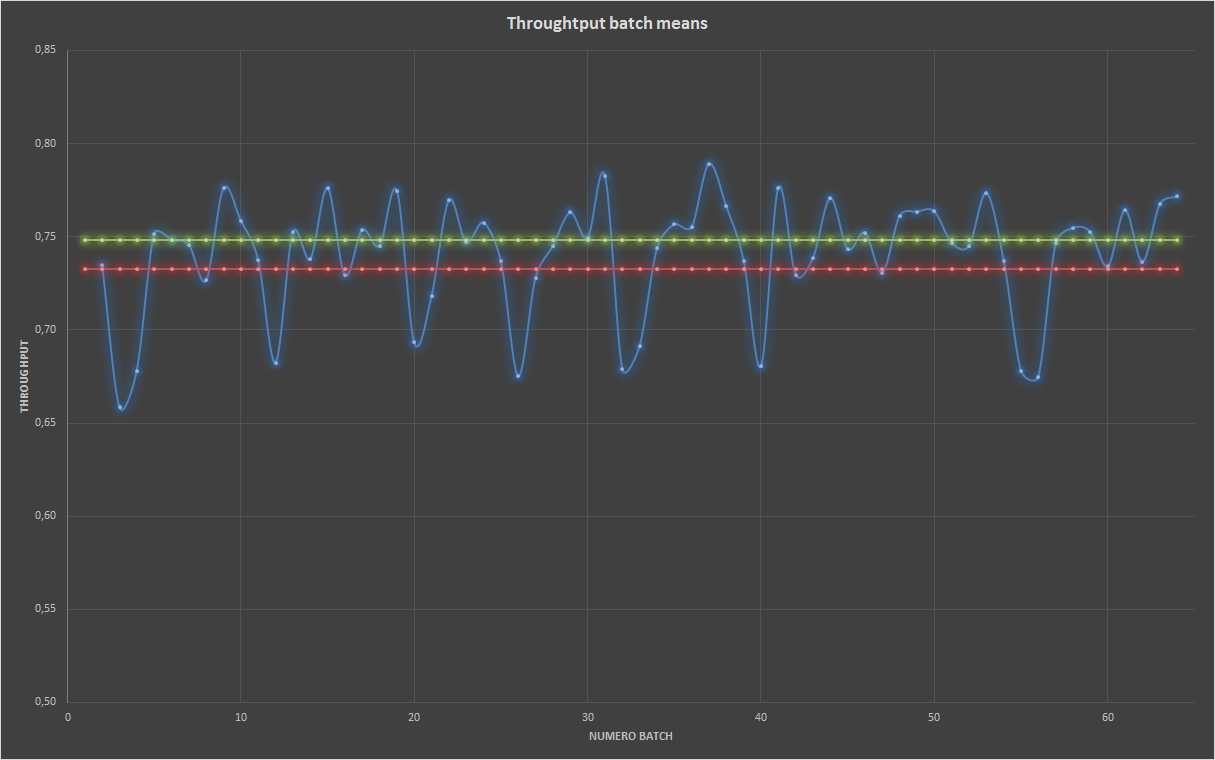
\includegraphics[scale=0.4]{img/throughputBM.png}
 \caption[Throughput nel caso dei batch means]{Throughput nel caso dei batch means}
 \label{fig:Throughput nel caso dei batch means}
\end{figure}

Nei primi batch possiamo vedere che il sistema ha tempi di risposta molto alti, che vanno a
diminuire nei batch successivi fino ad andarsi ad assestare, questo comportamento è dovuto al
fatto che il sistema all'inizio \'e in una fase transitoria, e quindi ancora deve stabilizzarsi.

La stessa analisi è stata effettuata anche per il throughtput, che per\`o risulta oscillare 
in maniera pi\`u o meno evidente; probabilmente tale comportamento \'e dovuto al meccanismo di
overload management che nel momento di attivazione permette al sistema di ``scaricarsi''.


\section{Conclusioni}

In questo progetto \'e stata effettuata l'analisi delle prestazioni di un 
sistema che emula uno scenario di traffico web reale.
Infatti oltre a simulare un comportamento stocastico riguardante sia i tempi di 
interarrivo delle 
richieste effettuate dai client che i loro tempi di processamento nei server e 
sia la loro fase di thinking. Inoltre fissati i parametri del sistema e 
sfruttando le specifiche riportate ed applicando il meccanismo di 
overload management, il sistema presenta un comportamento simile ai server web 
reali. 

Si \'e analizzato quindi le prestazioni di tale sistema al variare delle 
distribuzioni dei tempi di 
servizio, dell'applicazione del meccanismo di overload management valutando 
l'andamento 
degli indici di prestazione di interesse quali lo useful throughput e i tempi di 
risposta del 
sistema, oltre a valutare il drop ratio e l'abort ratio. A tale scopo \'e stato 
utilizzato un 
simulatore next-event il quale integra un meccanismo di avanzamento del tempo 
simulato 
basato sull'occorrenza degli eventi schedulati in apposite strutture dati.     % 9. Simulazioni
 	\chapter{Analisi dei risultati}

I grafici presentati sono il frutto delle simulazioni descritte precedentemente. Queste si dividono in quattro sezioni:

\begin{itemize}
 \item Analisi del caso in cui il Front-end abbia distribuzione esponenziale;
 \item Analisi del caso in cui il Front-end ha distribuzione 10 Erlang;
 \item Analisi del caso in cui il Front-end ha distribuzione iperesponenziale;
 \item Analisi del caso peggiore tra i tre sopra descritti con l'overload manager attivo.
\end{itemize}

\noindent Per ognuno di questi sono riportati i dati relativi a:
\begin{enumerate}
 \item Tempo di risposta medio del sistema;
 \item Throughput;
 \item Autocorrelazione.
\end{enumerate}

\section{Front server esponenziale}

\subsection{Tempo di risposta}
Per prima cosa analizziamo il tempo medio di risposta del sistema. Nella figura è rappresentato un grafico con i tempi medi ottenuti ogni 100 secondi di simulazione. Il sistema risulta essere \textbf{instabile}, in quanto i tempi crescono in modo praticamente lineare, questo risulta essere conseguenza del fatto che la cosa del Front server tende a crescere all'infinito.

\begin{figure}[H]
	\begin{center}
	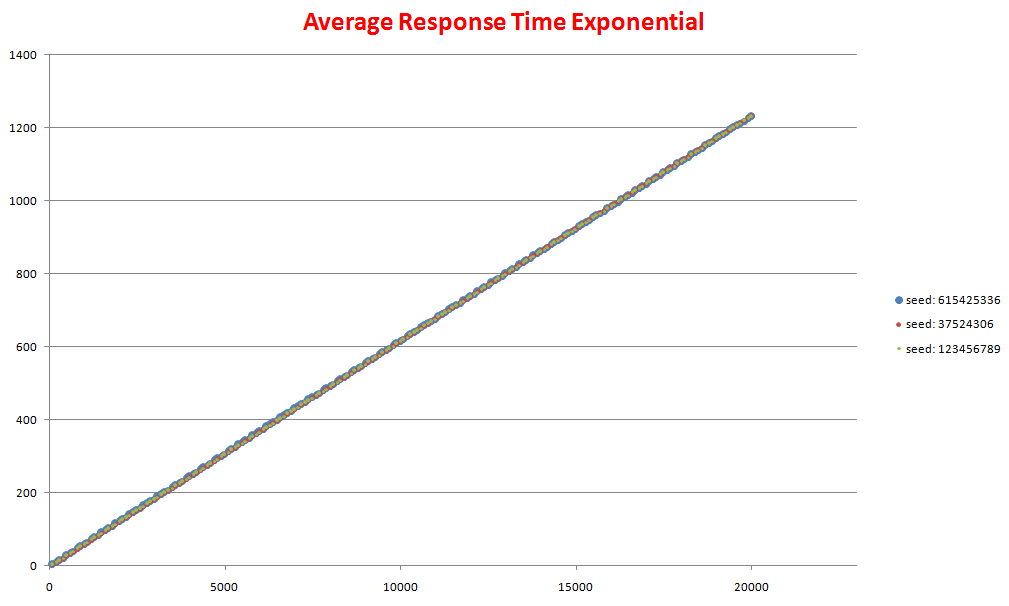
\includegraphics[scale=0.4]{img/exp_res_time.png}
	\caption[Tempo di risposta del sistema senza Overload Management (Legge Front-End:Esponenziale)]{Tempo di risposta del sistema nel caso di tempo di servizio esponenziale senza Overload Management.}
	\label{fig:exp_res_time}
	\end{center}
\end{figure}

\subsection{Throughput}
\begin{figure}[H]
	\begin{center}
	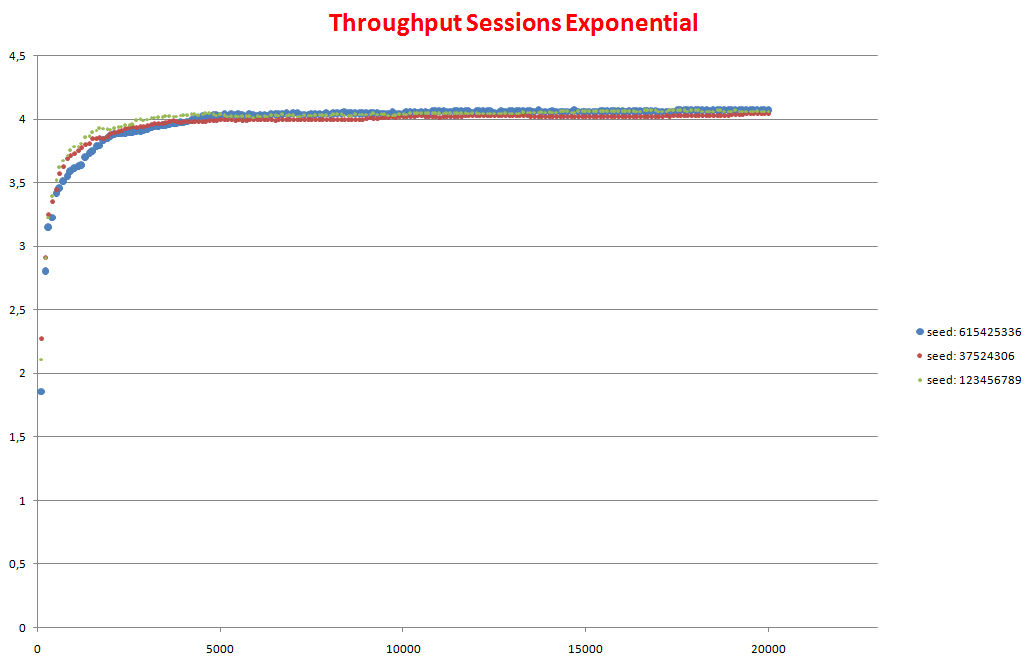
\includegraphics[scale=0.4]{img/exp_t_sess.png}
	\caption[Throughput del sistema senza Overload Management (Legge Front-End:Esponenziale)]{Througput del sistema nel caso di tempo di servizio esponenziale senza Overload Management.}
	\label{fig:exp_t_sess}
	\end{center}
\end{figure}
La seconda metrica di cui ci andiamo ad interessare è quella relativa al throughput. Come si evince dall'immagine c'è una saturazione molto veloce del front-end e infatti questo si stabilizza molto velocemente attorno al valore 4.

Un intervallo di confidenza per il throughput calcolato è il seguente:

\begin{center} IC = [3.96532859 - 0.02472767 ; 3.96532859 - 0.02472767] =  [3.94060091 ; 3.99005626]\end{center}

Mentre qui di seguito vediamo l'istogramma relativo a tale metrica:
\begin{figure}[H]
	\begin{center}
	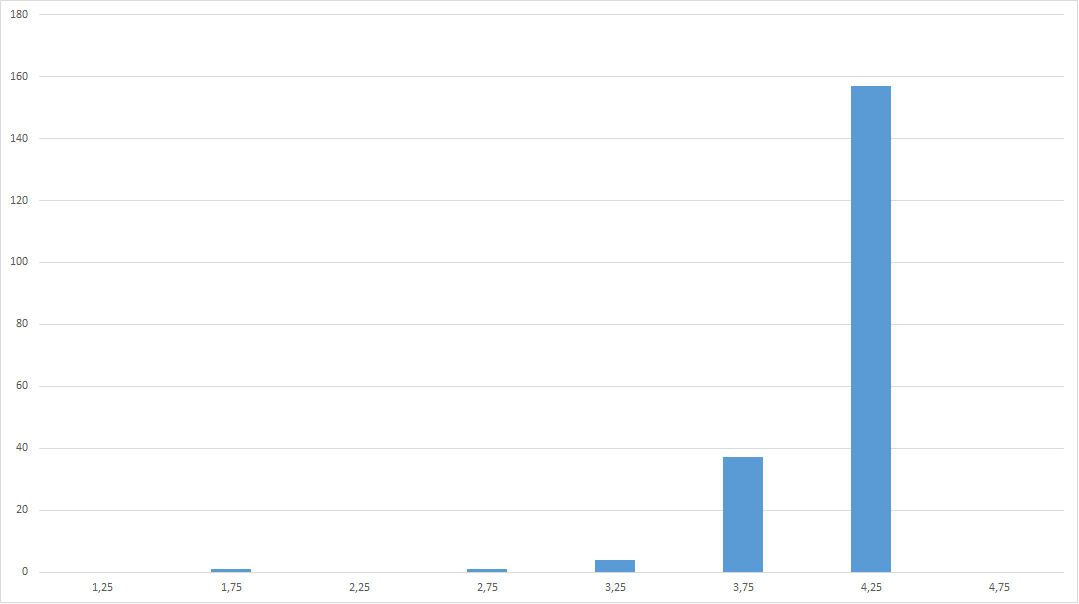
\includegraphics[scale=0.4]{img/histogram.png}
	\caption[Istogramma per il throughput]{Istogramma per il throughput.}
	\label{fig:exp_t_sess}
	\end{center}
\end{figure}

\section{Autocorrelazione}
L'ultima metrica da calcolare è quella relativa all'autocorrelazione. Vediamo sotto forma di tabella i risultati ottenuti per i diversi seed.
\begin{table}[H]
 \centering
 \begin{tabular}{|c|c|c|c|}
 \hline
 \# & SEED: 615425336 & SEED: 37524306 & SEED: 123456789 \\ \hline
 1 & 0,98995668 & 0,98997536 & 0,98994852 \\ \hline
 2 & 0,97981444 & 0,97985091 & 0,97979832 \\ \hline
 3 & 0,96957032 & 0,96962554 & 0,96954728 \\ \hline
 4 & 0,95922107 & 0,95930107 & 0,95919848 \\ \hline
 5 & 0,94876988 & 0,94887862 & 0,94875186 \\ \hline
 6 & 0,93821731 & 0,9383594 & 0,93820573 \\ \hline
 7 & 0,92757015 & 0,92773803 & 0,92755606 \\ \hline
 8 & 0,9168206 & 0,91701647 & 0,91680759 \\ \hline
 9 & 0,90597061 & 0,90619544 & 0,90596156 \\ \hline
 10 & 0,89501832 & 0,89527232 & 0,89501785 \\ \hline
 11 & 0,88396744 & 0,88424369 & 0,88398003 \\ \hline
 12 & 0,87281776 & 0,81311632 & 0,87284494 \\ \hline
 13 & 0,86157167 & 0,86189008 & 0,86161132 \\ \hline
 14 & 0,85022491 & 0,85056456 & 0,85027646 \\ \hline
 15 & 0,83877974 & 0,83913659 & 0,83884245 \\ \hline
 16 & 0,82723641 & 0,82760883 & 0,82730328 \\ \hline
 17 & 0,81559788 & 0,81597844 & 0,81566353 \\ \hline
 18 & 0,80385917 & 0,80424497 & 0,80392133 \\ \hline
 19 & 0,79202286 & 0,79241003 & 0,79208271 \\ \hline
 20 & 0,78008154 & 0,78047206 & 0,78014424 \\ \hline
 \end{tabular}
 \caption{Tabella esperimenti eseguiti per il front-end esponenziale}
 \end{table}
 
 \section{Confronto con altre distribuzioni}
 Il simulatore come già detto offre la possibilità di variare la distribuzione del front-end allo scopo di vedere le possibili variazioni di performance del sistema.
 Le distribuzioni utilizzate sono state le seguenti:
 \begin{itemize}
  \item Esponenziale
  \item 10 Erlang
  \item Iperesponenziale
 \end{itemize}
Per confrontare i vari casi di studio è stato utilizzato il tempo di risposta. In questo caso notiamo come ci sia un peggioramento delle condizioni nel caso la distribuzione usata sia la 10 Erlang, mentre nel caso dell'iperesponenziale abbiamo un comportamento molto simile all'esponenziale.
%\begin{figure}[H]
%	\begin{center}
%	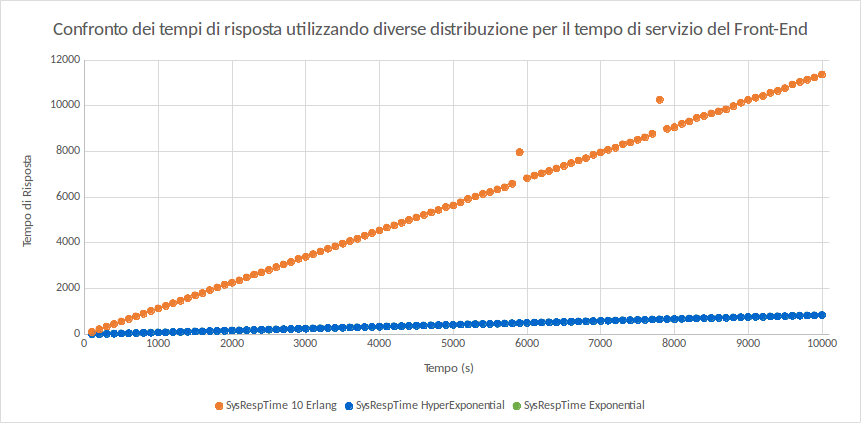
\includegraphics[scale=0.5]{img/confr_distrib.png}
%	\caption[Confronto tra i tempi di risposta]{Confronto tra i tempi di risposta.}
%	\label{fig:confr_distrib}
%	\end{center}
%\end{figure}

\section{Overload manager}
Osservando i risultati conseguiti nella sezione precedente è stato deciso di attivare il meccanismo di overload management sulla distribuzione 10 Erlang. Questo perchè tra le 3 distribuzioni ha mostrato l'andamento peggiore. Si è quindi effettuata una nuova analisi delle metriche prima illustrate.

\subsection{Tempo di risposta}
Il tempo di risposta del sistema quando è attivato questo meccanismo tende a scendere rispetto a prima e risulta arrivare quasi ad una stabilità. Questa stabilità però non è proprio reale in quanto il sistema \textit{oscilla} attorno a questo valore, anche a causa del fatto che le sessioni già accettate vengono abortite.

\begin{figure}[H]
	\begin{center}
	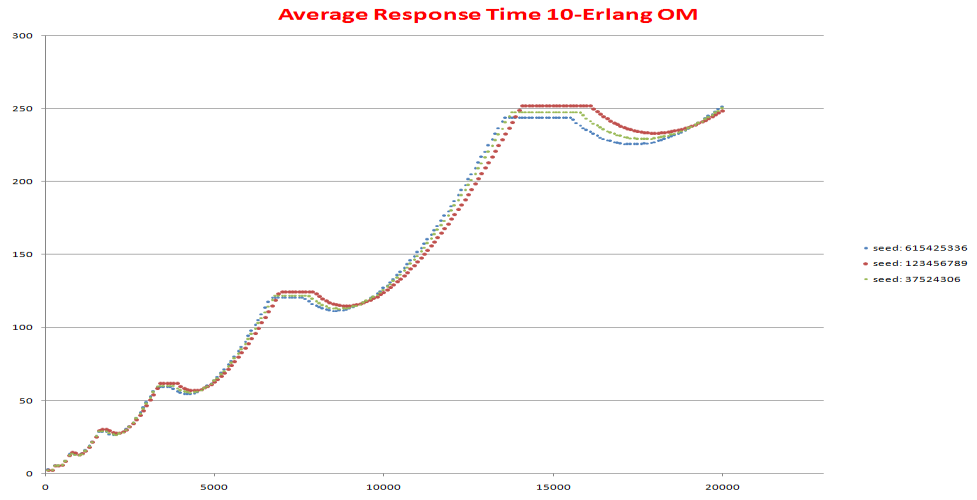
\includegraphics[scale=0.4]{img/er_om_res_time.png}
	\caption[Tempo di risposta del sistema nel caso di una 10 Erlang con overload manager]{Tempo di risposta del sistema nel caso di una 10 Erlang con overload manager.}
	\label{fig:erl_om_res_time}
	\end{center}
\end{figure}

\subsection{Throughput}
\begin{figure}[H]
	\begin{center}
	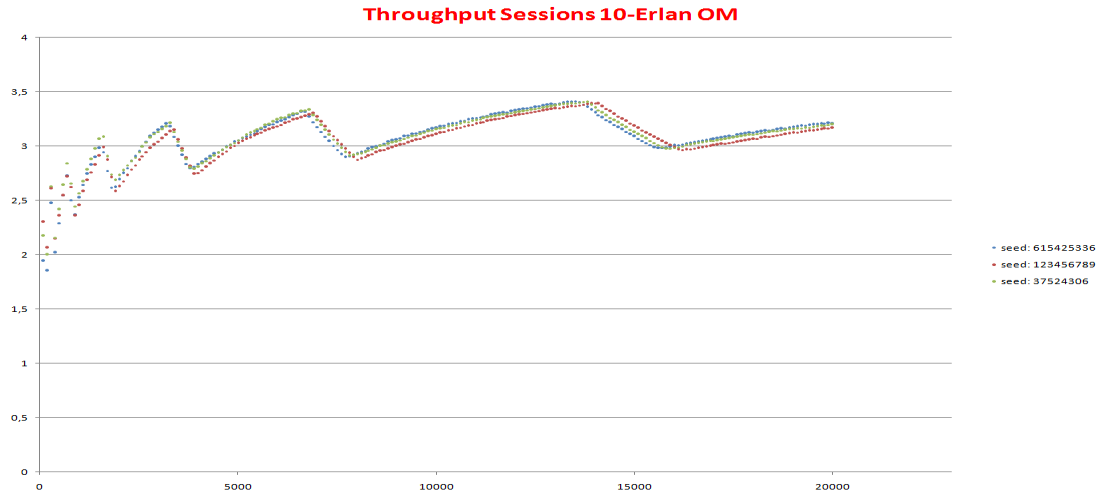
\includegraphics[scale=0.4]{img/erl_om_t.png}
	\caption[Throughput nel caso di una 10 Erlang con overload manager]{Throughput nel caso di una 10 Erlang con overload manager.}
	\label{fig:erl_om_t}
	\end{center}
\end{figure}
Per il throughput osserviamo lo stesso effetto descritto precedentemente in quanto si assesta attorno ad un valore però senza mai fermarsi del tutto, bensì oscillandovi attorno.



\subsection{Drop Ratio}
Il drop ratio misura il rapporto tra le sessioni rifiutate dal sistema e il numero di sessioni totali (ovvero accettate + rifiutate).
Notiamo che questo numero si assesta intorno al 30\% e questo accade poichè vengono rifiutate anche le connessioni già presenti, ciò permette al sistema di scendere molto velocemente sotto il 75\% di utilizzazione e riprendere dunque un normale funzionamento.
\begin{figure}[H]
	\begin{center}
	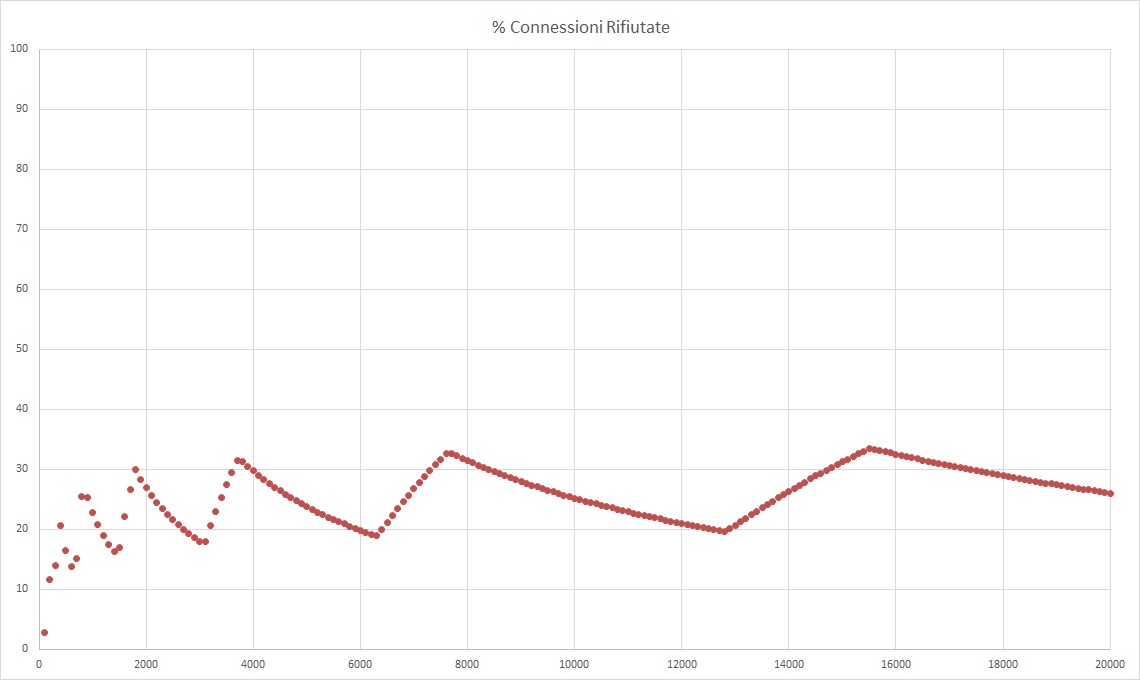
\includegraphics[scale=0.4]{img/Drop_ratio.png}
	\caption[Percentuale di connessioni rifiutate dal sistema.]{Percentuale di connessioni rifiutate dal sistema.}
	\label{fig:confr_distrib}
	\end{center}
\end{figure}

\subsection{Abort Ratio}
Nel caso di overload manager attivo il nostro simulatore deve impedire ad \textbf{ogni richiesta} di potersi mettere in coda al Front Server.
A causa di questo vincolo l'abort ratio è diverso da zero poichè questo si riferisce alle sessioni che vengono chiuse pur essendo state precedentemente accettate dal sistema. Come si può vedere dal grafico la percentuale di connessioni abortite dal sistema è abbastanza elevato.
\begin{figure}[H]
	\begin{center}
	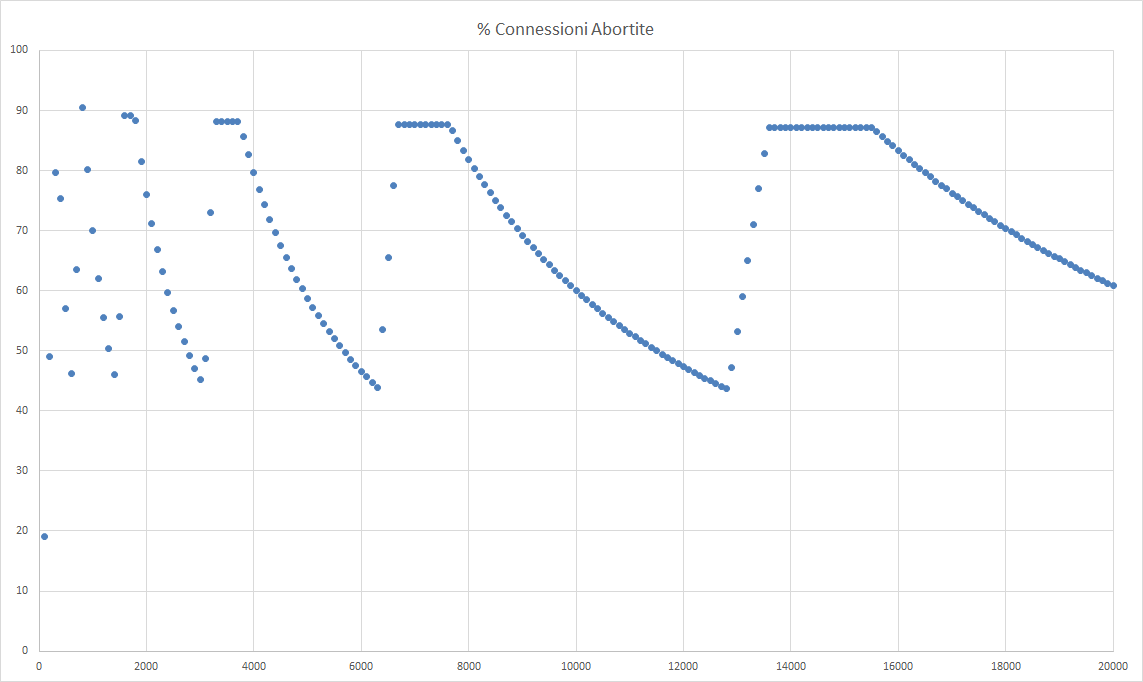
\includegraphics[scale=0.4]{img/abort_ratio.png}
	\caption[Percentuale di connessioni abortite dal sistema.]{Percentuale di connessioni abortite dal sistema.}
	\label{fig:confr_distrib}
	\end{center}
\end{figure}
    % 10. Analisi dei Risultati

 	\appendix
 	\chapter{Codice}
	\label{appendix:codice}

\definecolor{dkgreen}{rgb}{0,0.6,0}
\definecolor{gray}{rgb}{0.5,0.5,0.5}
\definecolor{mauve}{rgb}{0.58,0,0.82}

\lstset{frame=tb,
  language=C,
  aboveskip=3mm,
  belowskip=3mm,
  showstringspaces=false,
  columns=flexible,
  basicstyle={\scriptsize\ttfamily},
  numbers=none,
  numberstyle=\scriptsize\color{gray},
  keywordstyle=\color{blue},
  commentstyle=\color{dkgreen},
  stringstyle=\color{mauve},
  breaklines=true,
  breakatwhitespace=true,
  tabsize=2
}

\section{Test degli estremi}
\subsection{test.c}
\lstinputlisting[breaklines]{./codice/lehmer/test.c}

\section{Intervalli di Confidenza}
\subsection{interval\_calculator.c}
\lstinputlisting[breaklines]{./codice/ic/ic.c}

\section{Autocorrelazione}
\subsection{autocorrelation.c}
\lstinputlisting[breaklines]{./codice/autocorrelazione/autocorrelation.c}

\section{Simulatore}
\subsection{simulatore.c}
\lstinputlisting[breaklines]{./codice/simulatore.c}

\subsection{arrival\_queue.h}
\lstinputlisting[breaklines]{./codice/arrival_queue.h}

\subsection{client\_req.h}
\lstinputlisting[breaklines]{./codice/client_req.h}

\subsection{event\_list.h}
\lstinputlisting[breaklines]{./codice/event_list.h}

\subsection{event\_manager.c}
\lstinputlisting[breaklines]{./codice/event_manager.c}

\subsection{file\_manager.c}
\lstinputlisting[breaklines]{./codice/file_manager.c}

\subsection{generate\_random\_value.h}
\lstinputlisting[breaklines]{./codice/generate_random_value.h}

\subsection{global\_variables.h}
\lstinputlisting[breaklines]{./codice/global_variables.h}

\subsection{req\_queue.h}
\lstinputlisting[breaklines]{./codice/req_queue.h}

\subsection{rng.c}
\lstinputlisting[breaklines]{./codice/rng.c}

\subsection{rng.h}
\lstinputlisting[breaklines]{./codice/rng.h}

\subsection{rvms.c}
\lstinputlisting[breaklines]{./codice/rvms.c}

\subsection{rvms.h}
\lstinputlisting[breaklines]{./codice/rvms.h}

\subsection{simulation\_type.h}
\lstinputlisting[breaklines]{./codice/simulation_type.h}

\subsection{user\_signal.c}
\lstinputlisting[breaklines]{./codice/user_signal.c}

\subsection{utils.h}
\lstinputlisting[breaklines]{./codice/utils.h}
      % Codice sorgente
	\chapter{Grafici} 
\label{appendix:grafici}
\section{Distribuzione 10 Erlang}
\begin{comment}
\begin{figure}[H]
	\begin{center}
	\includegraphics[scale=0.5]{grafici_10-Erlang/AverageResponseTime.png}
	\caption[Tempo di risposta del sistema senza Overload Management (Legge Front-End:10 Erlang)]{Tempo di risposta del sistema senza Overload Management (Legge Front-End:10 Erlang).}
	\label{fig:exp_res_time}
	\end{center}
\end{figure}

\begin{figure}[H]
	\begin{center}
	\includegraphics[scale=0.5]{grafici_10-Erlang/ThroughputSessions.png}
	\caption[Throughput del sistema senza Overload Management (Legge Front-End:10 Erlang)]{Throughput del sistema senza Overload Management (Legge Front-End:10 Erlang).}
	\label{fig:exp_res_time}
	\end{center}
\end{figure}
\end{comment}
\section{Distribuzione Iperesponenziale}
\begin{comment}
\begin{figure}[H]
	\begin{center}
	\includegraphics[scale=0.5]{grafici_Hyperexponential/AverageResponseTime.png}
	\caption[Tempo di risposta del sistema senza Overload Management (Legge Front-End:Iperesponenziale)]{Tempo di risposta del sistema senza Overload Management (Legge Front-End:Iperesponenziale).}
	\label{fig:exp_res_time}
	\end{center}
\end{figure}

\begin{figure}[H]
	\begin{center}
	\includegraphics[scale=0.5]{grafici_Hyperexponential/ThroughputSessions.png}
	\caption[Throughput del sistema senza Overload Management (Legge Front-End:Iperesponenziale)]{Throughput del sistema senza Overload Management (Legge Front-End:Iperesponenziale).}
	\label{fig:exp_res_time}
	\end{center}
\end{figure}
\end{comment}
\section{Grafici delle autocorrelazioni}
\begin{comment}
\begin{figure}[H]
	\begin{center}
	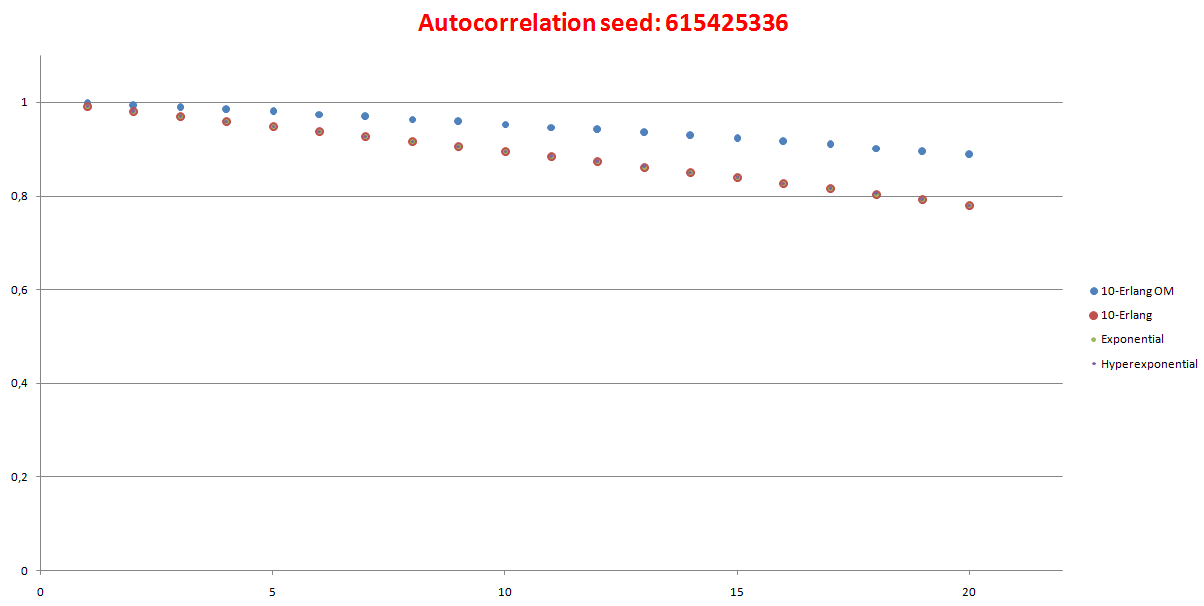
\includegraphics[scale=0.5]{grafici_Autocorrelazione/seed625435336.png}
	\caption[Autocorrelazione per il seed 625435336]{Autocorrelazione per il seed 625435336.}
	\label{fig:exp_res_time}
	\end{center}
\end{figure}
\begin{figure}[H]
	\begin{center}
	\includegraphics[scale=0.5]{grafici_Autocorrelazione/ThroughputSessions.png}
	\caption[Throughput del sistema senza Overload Management (Legge Front-End:Iperesponenziale)]{Throughput del sistema senza Overload Management (Legge Front-End:Iperesponenziale).}
	\label{fig:exp_res_time}
	\end{center}
\end{figure}

\begin{figure}[H]
	\begin{center}
	\includegraphics[scale=0.5]{grafici_Autocorrelazione/ThroughputSessions.png}
	\caption[Throughput del sistema senza Overload Management (Legge Front-End:Iperesponenziale)]{Throughput del sistema senza Overload Management (Legge Front-End:Iperesponenziale).}
	\label{fig:exp_res_time}
	\end{center}
\end{figure}
\end{comment}
\section{Distribuzione 10 Erlang con Overload Manager}
\begin{comment}
\begin{figure}[H]
	\begin{center}
	\includegraphics[scale=0.5]{grafici_10-Erlang_OM/AverageResponseTime.png}
	\caption[Tempo di risposta del sistema con Overload Management (Legge Front-End:10-Erlang)]
	{Tempo di risposta del sistema con Overload Management (Legge Front-End:10-Erlang)}
	\label{fig:exp_res_time}
	\end{center}
	\end{figure}

\begin{figure}[H]
	\begin{center}
	\includegraphics[scale=0.5]{grafici_10-Erlang_OM/ThroughputSessions.png}
	\caption[Throughput di risposta del sistema con Overload Management (Legge Front-End:10-Erlang)]
	{Throughput di risposta del sistema con Overload Management (Legge Front-End:10-Erlang)}
	\label{fig:exp_res_time}
	\end{center}
	\end{figure}
\end{comment}
\section{Distribuzione Esponenziale}
\begin{comment}
\begin{figure}[H]
\begin{center}
	
	\includegraphics[scale=0.5]{grafici_Exponential/AverageResponseTime.png}
	\caption[Tempo di risposta del sistema senza Overload Management (Legge Front-End:Esponenziale)]
	{Tempo di risposta del sistema senza Overload Management (Legge Front-End:Esponenziale)}
	\label{fig:exp_res_time}
	\end{center}
	\end{figure}
	
\begin{figure}[H]
	
\begin{center}
	\includegraphics[scale=0.5]{grafici_Exponential/ThroughputSessions.png}
	\caption[Throughput del sistema senza Overload Management (Legge Front-End:Esponenziale)]
	{Tempo di risposta del sistema senza Overload Management (Legge Front-End:Esponenziale)}
	\label{fig:exp_res_time}
	\end{center}
	\end{figure}
\end{comment}
\section{Grafici delle autocorrelazioni}
\begin{comment}
\begin{figure}[H]
	\begin{center}
	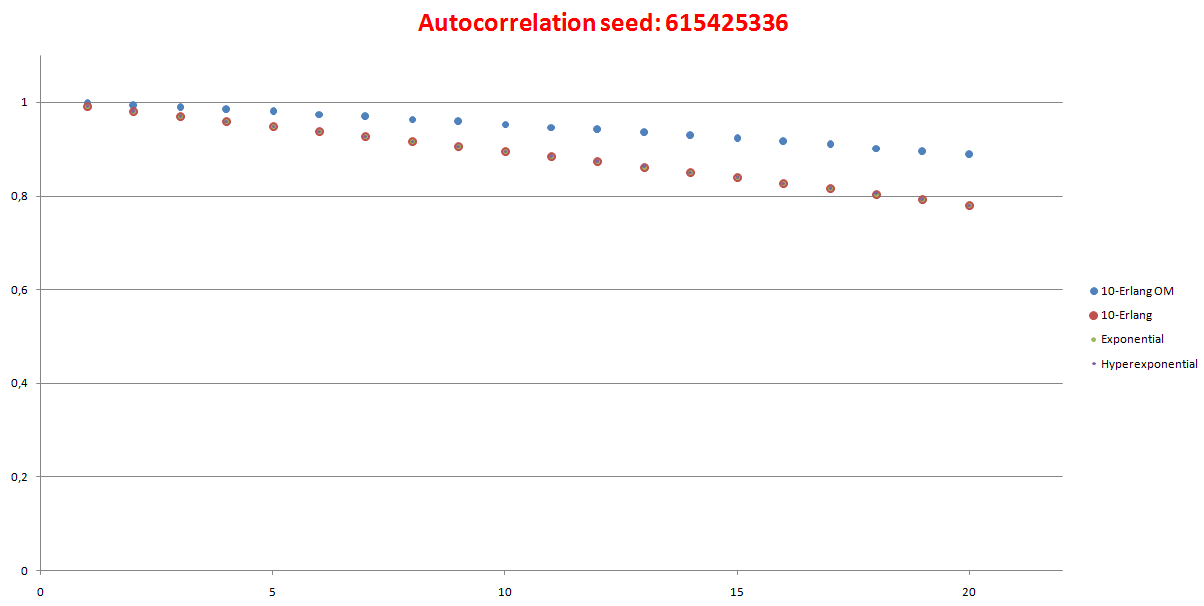
\includegraphics[scale=0.5]{grafici_Autocorrelazione/seed625435336.png}
	\caption[Autocorrelazione per il seed 625435336]{Autocorrelazione per il seed 625435336.}
	\label{fig:exp_res_time}
	\end{center}
\end{figure}

\begin{figure}[H]
	\begin{center}
	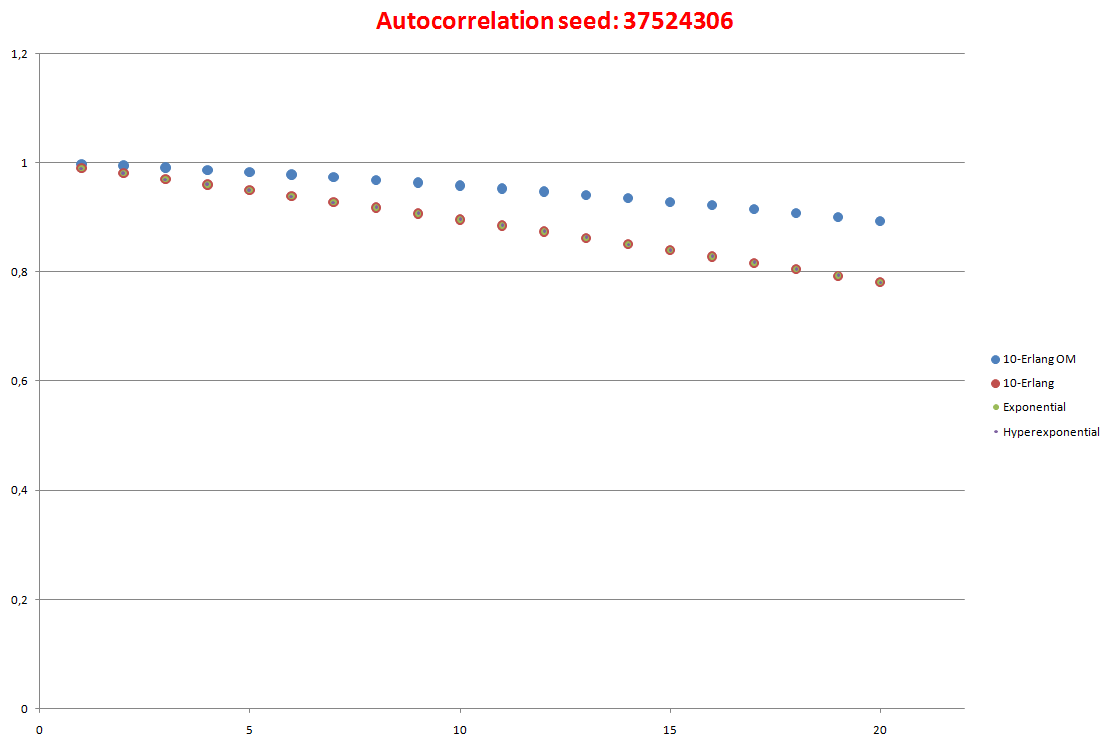
\includegraphics[scale=0.6]{grafici_Autocorrelazione/seed37524306.png}
	\caption[Autocorrelazione per il seed 37524306]{Autocorrelazione per il seed 37524306.}
	\label{fig:exp_res_time}
	\end{center}
\end{figure}

\begin{figure}[H]
	\begin{center}
	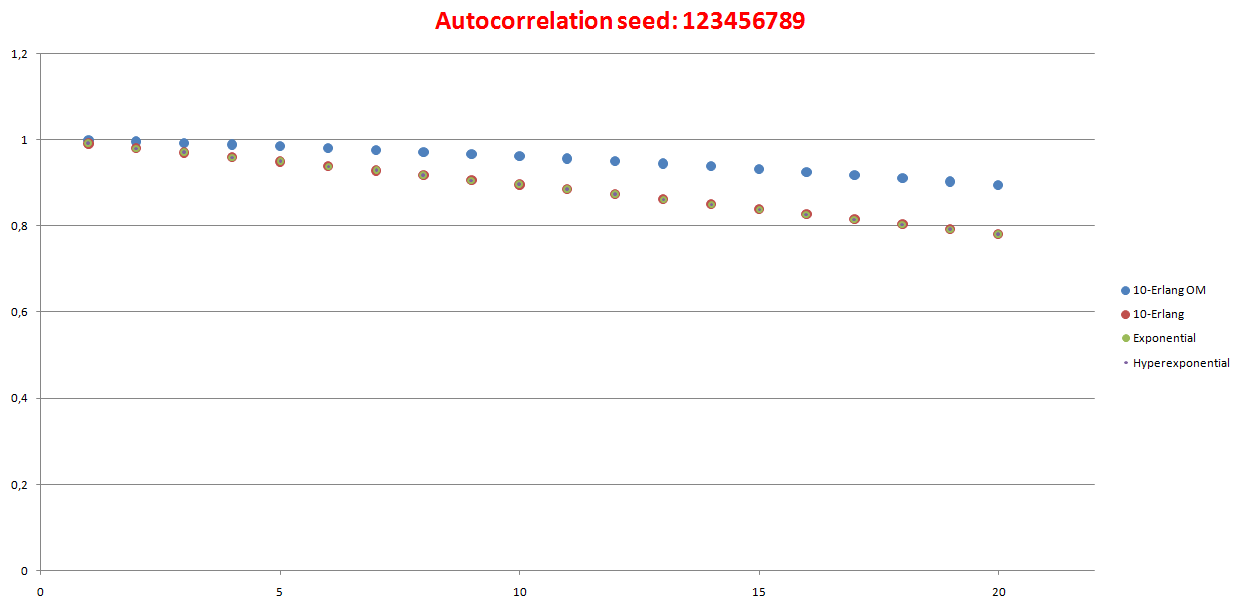
\includegraphics[scale=0.5]{grafici_Autocorrelazione/seed123456789.png}
	\caption[Autocorrelazione per il seed 123456789]{Autocorrelazione per il seed 123456789.}
	\label{fig:exp_res_time}
	\end{center}
\end{figure}
\end{comment} 	   % Grafici dei test
 \end{document} 
